\documentclass[letterpaper, 10 pt, conference]{article} 
\usepackage[english]{babel}
\usepackage{amsmath,amssymb,amscd,amsthm} % variety of useful math macros
\usepackage[inner=1.5 cm, outer = 1.5 cm, top=1 cm, bottom = 1.5 cm]{geometry}
\usepackage{subcaption}
%For inserting graphics
\usepackage{graphicx}
\usepackage[dvipsnames]{xcolor}
\usepackage{listings}
\usepackage[utf8]{inputenc}
\usepackage{hyperref}
\usepackage{array, multirow}
\usepackage{lipsum}
\usepackage{natbib}

\bibliographystyle{abbrvnat}

\newtheorem{thm}{Theorem}
\newtheorem{prop}{Proposition}
\newtheorem{lemma}{Lemma}
\newtheorem{ex}{Exercise}

\newcommand\ql{\textquotedblleft}
\newcommand\qr{\textquotedblright}


\newcommand\E{\ensuremath{\mathbb{E}}}
\newcommand\N{\ensuremath{\mathbb{N}}}
\renewcommand{\P}{\ensuremath{\mathbb{P}}}
\newcommand\Q{\ensuremath{\mathbb{Q}}}
\newcommand\R{\ensuremath{\mathbb{R}}}
\newcommand\Z{\ensuremath{\mathbb{Z}}}

\newcommand\V{\ensuremath{\mathrm{Var}}}
\newcommand\Om{\ensuremath{\Omega}}
\newcommand{\w}{\ensuremath{\omega}}

\title{Computer simulated exercises
}

\hypersetup{
	colorlinks=true,
	linkcolor=blue,
	filecolor=magenta,      
	urlcolor=blue,
	citecolor=MidnightBlue
}

\renewcommand{\qedsymbol}{}

\lstset{ 
	backgroundcolor=\color{white},   % choose the background color; you must add \usepackage{color} or \usepackage{xcolor}; should come as last argument
	basicstyle=\footnotesize,        % the size of the fonts that are used for the code
	breakatwhitespace=false,         % sets if automatic breaks should only happen at whitespace
	breaklines=true,                 % sets automatic line breaking
	%captionpos=b,                    % sets the caption-position to bottom
	commentstyle=\color{PineGreen},    % comment style
	deletekeywords={...},            % if you want to delete keywords from the given language
	escapeinside={\%*}{*)},          % if you want to add LaTeX within your code
	extendedchars=true,              % lets you use non-ASCII characters; for 8-bits encodings only, does not work with UTF-8
	firstnumber=1,                % start line enumeration with line 1000
	frame=single,	                   % adds a frame around the code
	keepspaces=true,                 % keeps spaces in text, useful for keeping indentation of code (possibly needs columns=flexible)
	keywordstyle=\color{black},       % keyword style
	language=R,                 % the language of the code
	morekeywords={*,...},            % if you want to add more keywords to the set
	numbers=none,                    % where to put the line-numbers; possible values are (none, left, right)
	numbersep=5pt,                   % how far the line-numbers are from the code
	numberstyle=\tiny\color{gray}, % the style that is used for the line-numbers
	rulecolor=\color{black},         % if not set, the frame-color may be changed on line-breaks within not-black text (e.g. comments (green here))
	showspaces=false,                % show spaces everywhere adding particular underscores; it overrides 'showstringspaces'
	showstringspaces=false,          % underline spaces within strings only
	showtabs=false,                  % show tabs within strings adding particular underscores
	stepnumber=2,                    % the step between two line-numbers. If it's 1, each line will be numbered
	stringstyle=\color{purple},     % string literal style
	tabsize=2,	                   % sets default tabsize to 2 spaces
	title=\lstname                   % show the filename of files included with \lstinputlisting; also try caption instead of title
}

\author{G. Palafox}

\begin{document}
\maketitle
In the following, exercises from the book of \citet{snell} are simulated computationally on a Jupyter \citep{jupyter} notebook\footnote{The notebook with the code for the experiments, as well as this report, can be found in the Github Repository: \url{https://github.com/palafox794/AppliedProbabilityModels/tree/master/Assignment10}} with R \citep{R}.

\begin{ex}[Ex. 19, p. 249]\label{ex:subset-answers}
	A multiple choice exam is given. A problem has four possible answers, and exactly one answer is correct. The student is allowed to choose a subset of the four possible answers as his answer. If his chosen subset contains the correct answer, the student receives three points, but he loses one point for each wrong answer in his chosen subset. Show that if he just guesses a subset uniformly and randomly his expected score is zero. 
\end{ex}
\begin{proof}[Computer simulation]
The exercise is simulated as follows. A vector of possible answers, \texttt{a, b, c, d} is created. One of these is randomly selected as the correct answer. Then a random subset is taken from the possible answers, and a score is computed as per the rules laid out in the exercise. This is repeated 10,000 times to calculate the average score. The computation was done using the code in Listing \ref{lst:subset-answers}. On average, the score obtained is $-0.0129$, which is close to zero. A boxplot of the scores can be seen in Figure \ref{fig:subset-answers}.

 \begin{figure}
	\centering
	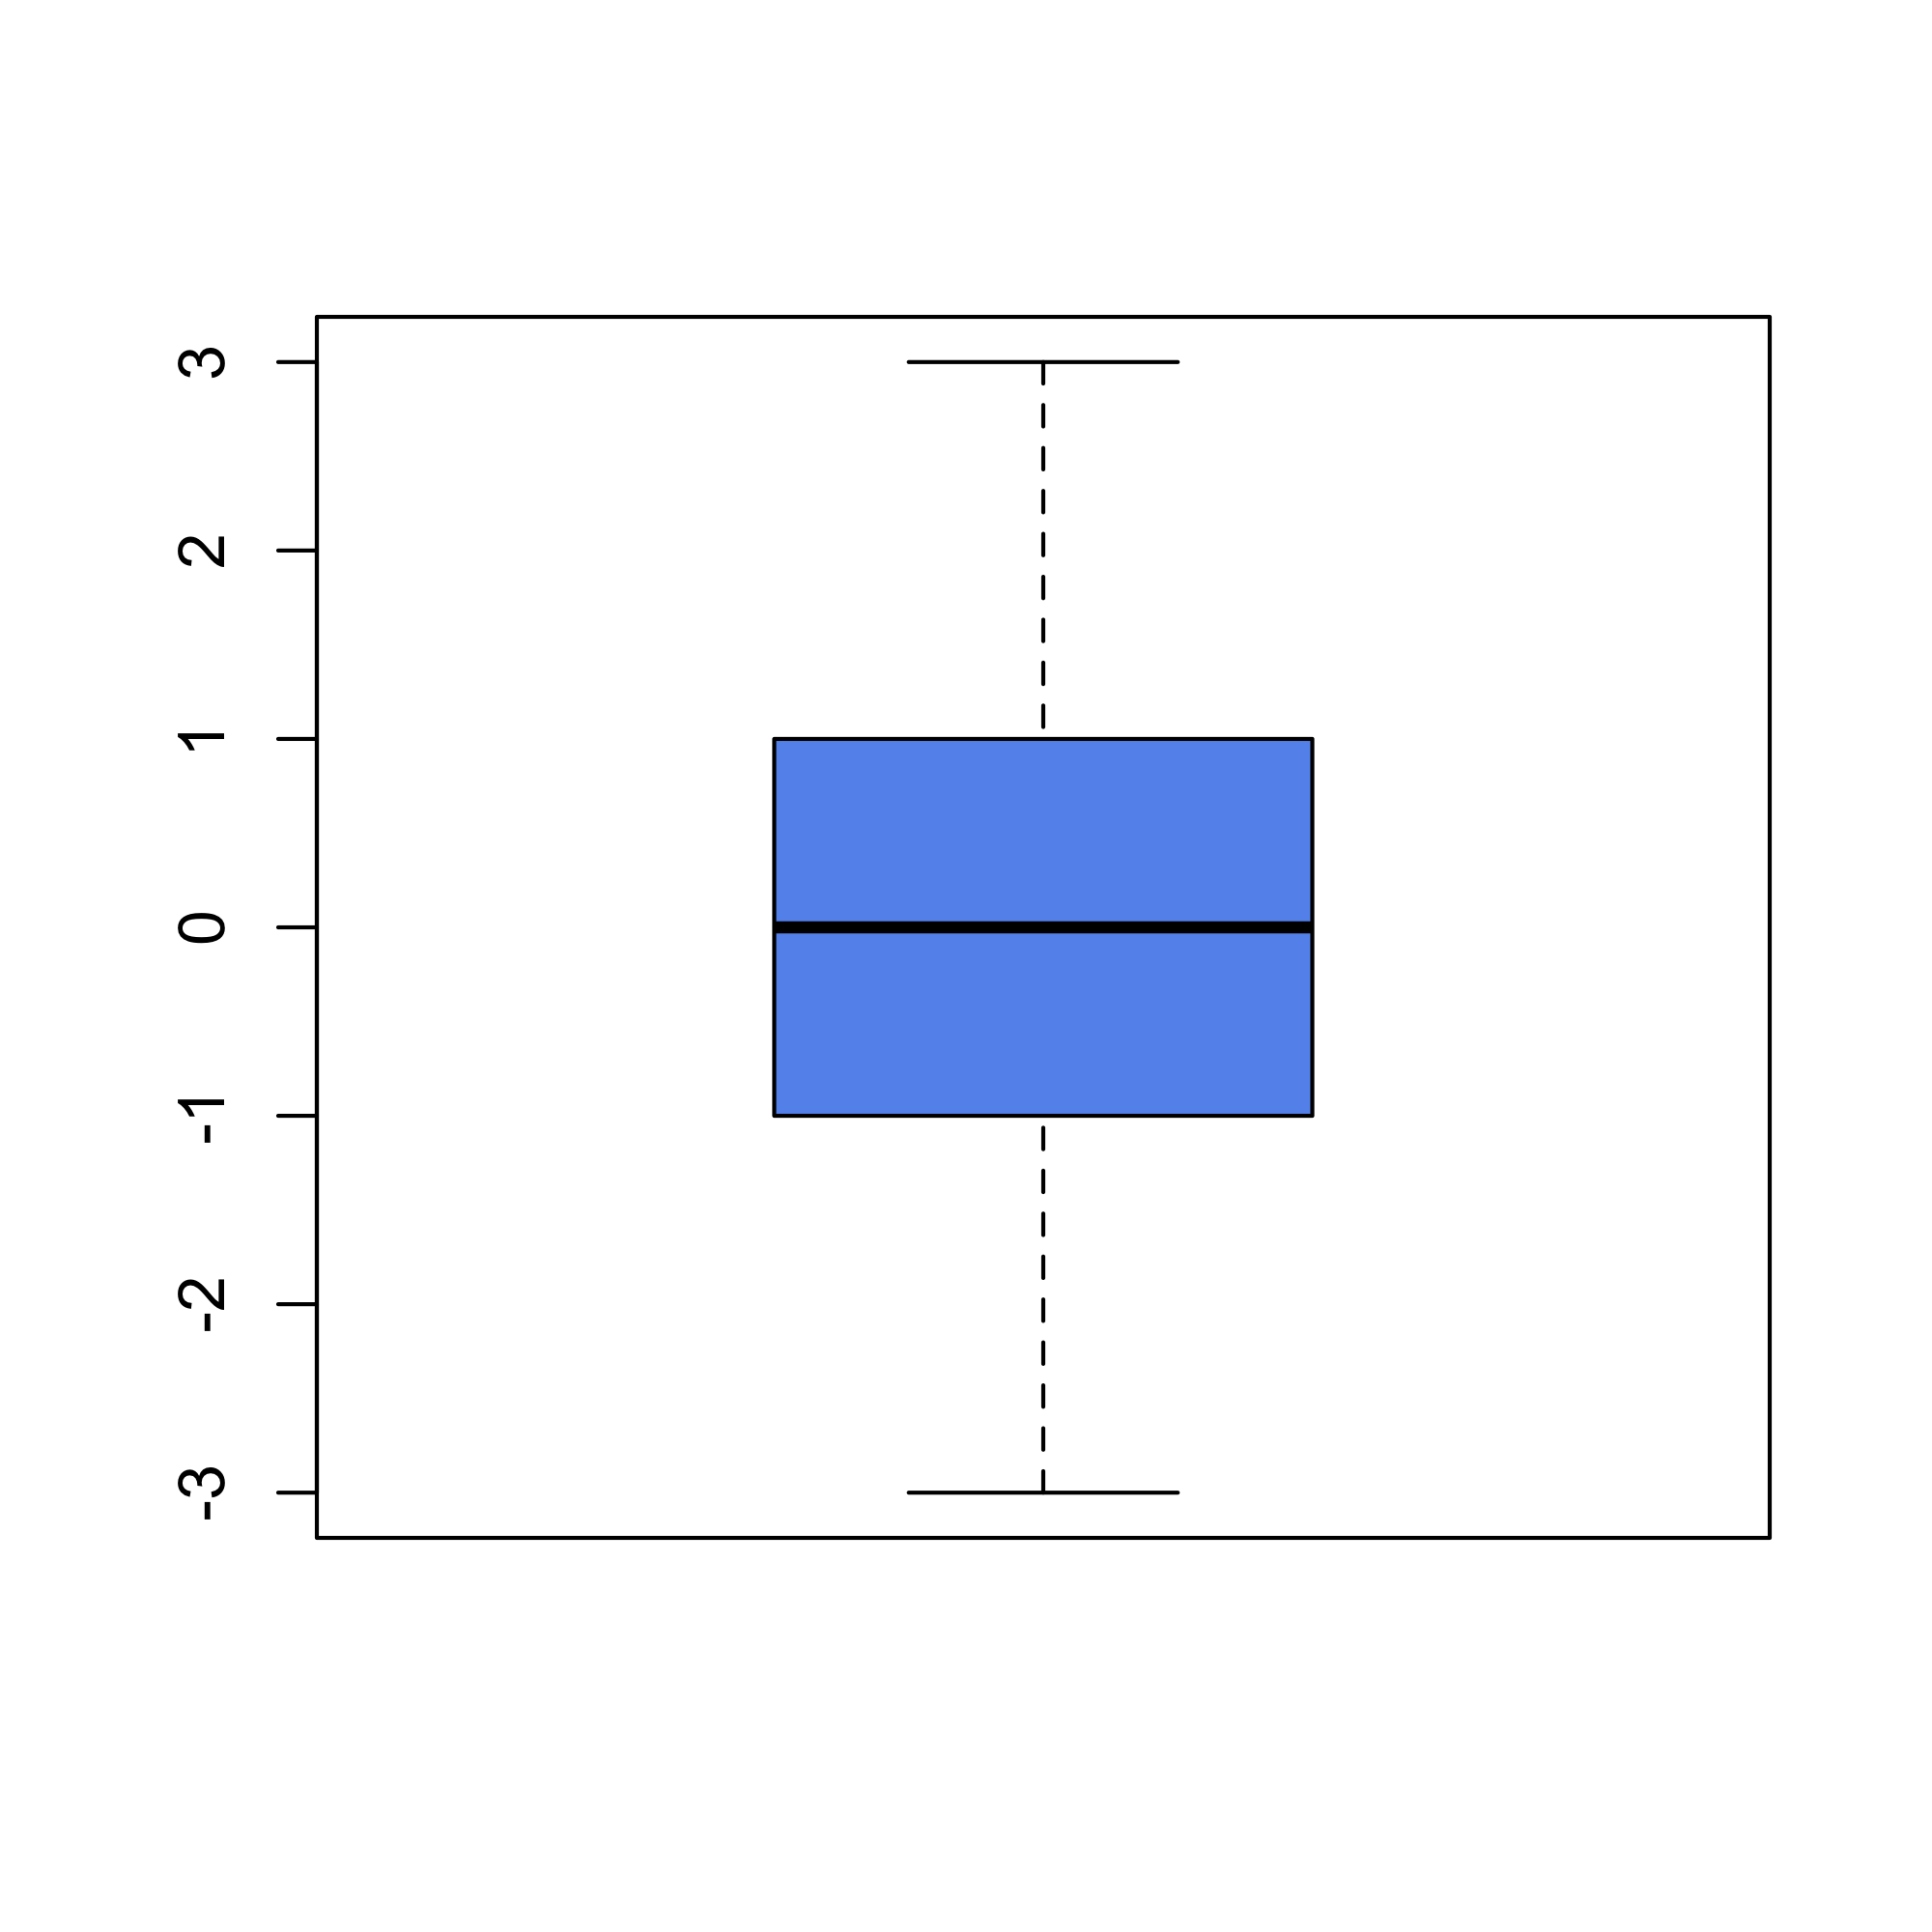
\includegraphics[width=0.35\linewidth]{scores}
	\caption{Scores obtained in experiment for Exercise \ref{ex:subset-answers}.}
	\label{fig:subset-answers}
\end{figure}

\begin{lstlisting}[language=R, caption={Code for Exercise \ref{ex:subset-answers}.}, label={lst:subset-answers} ]
answers = c('a', 'b', 'c', 'd')

scores <- numeric()

for(i in 1:10000){

correct_answer <- sample(answers, 1)

answerset <- sample(answers, sample(c(1,2,3,4), 1))

if (correct_answer %in% answerset){
	score <- 3 - (length(answerset)-1)
}else{
	score <- -length(answerset)
}

scores <- c(scores, score)
}
\end{lstlisting}
\end{proof}



\begin{ex}[Ex. 12, p. 264]\label{ex:standardized}
	Let $X$ be a random variable with $\mu = \E(X)$ and $\sigma^2 = \V(X)$. Define $X^\ast = (X-\mu)/\sigma$. The random variable $X^\ast$ is called the \textit{standardized random variable} associated with $X$. Show that this standardized random variable has expected value 0 and variance 1.
\end{ex}
\begin{proof}[Computer simulation]
	A thousand numbers following some specific distribution are generated. Their mean and variance is calculated. Then, the numbers are \textit{standardized} as the exercise suggests, and the mean and variance are re-calculated. The mean and variance of the original and standardized values are stored, and this is repeated a thousand times. The code in Listing \ref{lst:standardized} shows a function for standardizing a vector, and the experiment performed for uniformly distributed numbers. The experiment was also performed for normal (mean 1, standard deviation 0.5) distributed numbers, and for exponential distributed numbers with rate 10.  It can be seen in Figure \ref{fig:standardized} that the mean always shifts to zero, and variance always shifts to one, as expected.
	
	\begin{lstlisting}[language=R, caption={Code for Exercise \ref{ex:standardized}.}, label={lst:standardized} ]
standardize <- function(vector){
	return ((vector - mean(vector))/sqrt(var(vector)))
}

means_unif <- numeric()
means_unif_std <- numeric()

var_unif <- numeric()
var_unif_std <- numeric()

for(i in 1:1000){
	x <- runif(1000)

	means_unif <- c(means_unif, mean(x))
	means_unif_std <- c(means_unif_std, mean(standardize(x)))

	var_unif <- c(var_unif, var(x))
	var_unif_std <- c(var_unif_std, var(standardize(x))) 

}
	\end{lstlisting}
	
	\begin{figure}
		\centering
		\begin{subfigure}{0.3\linewidth}
			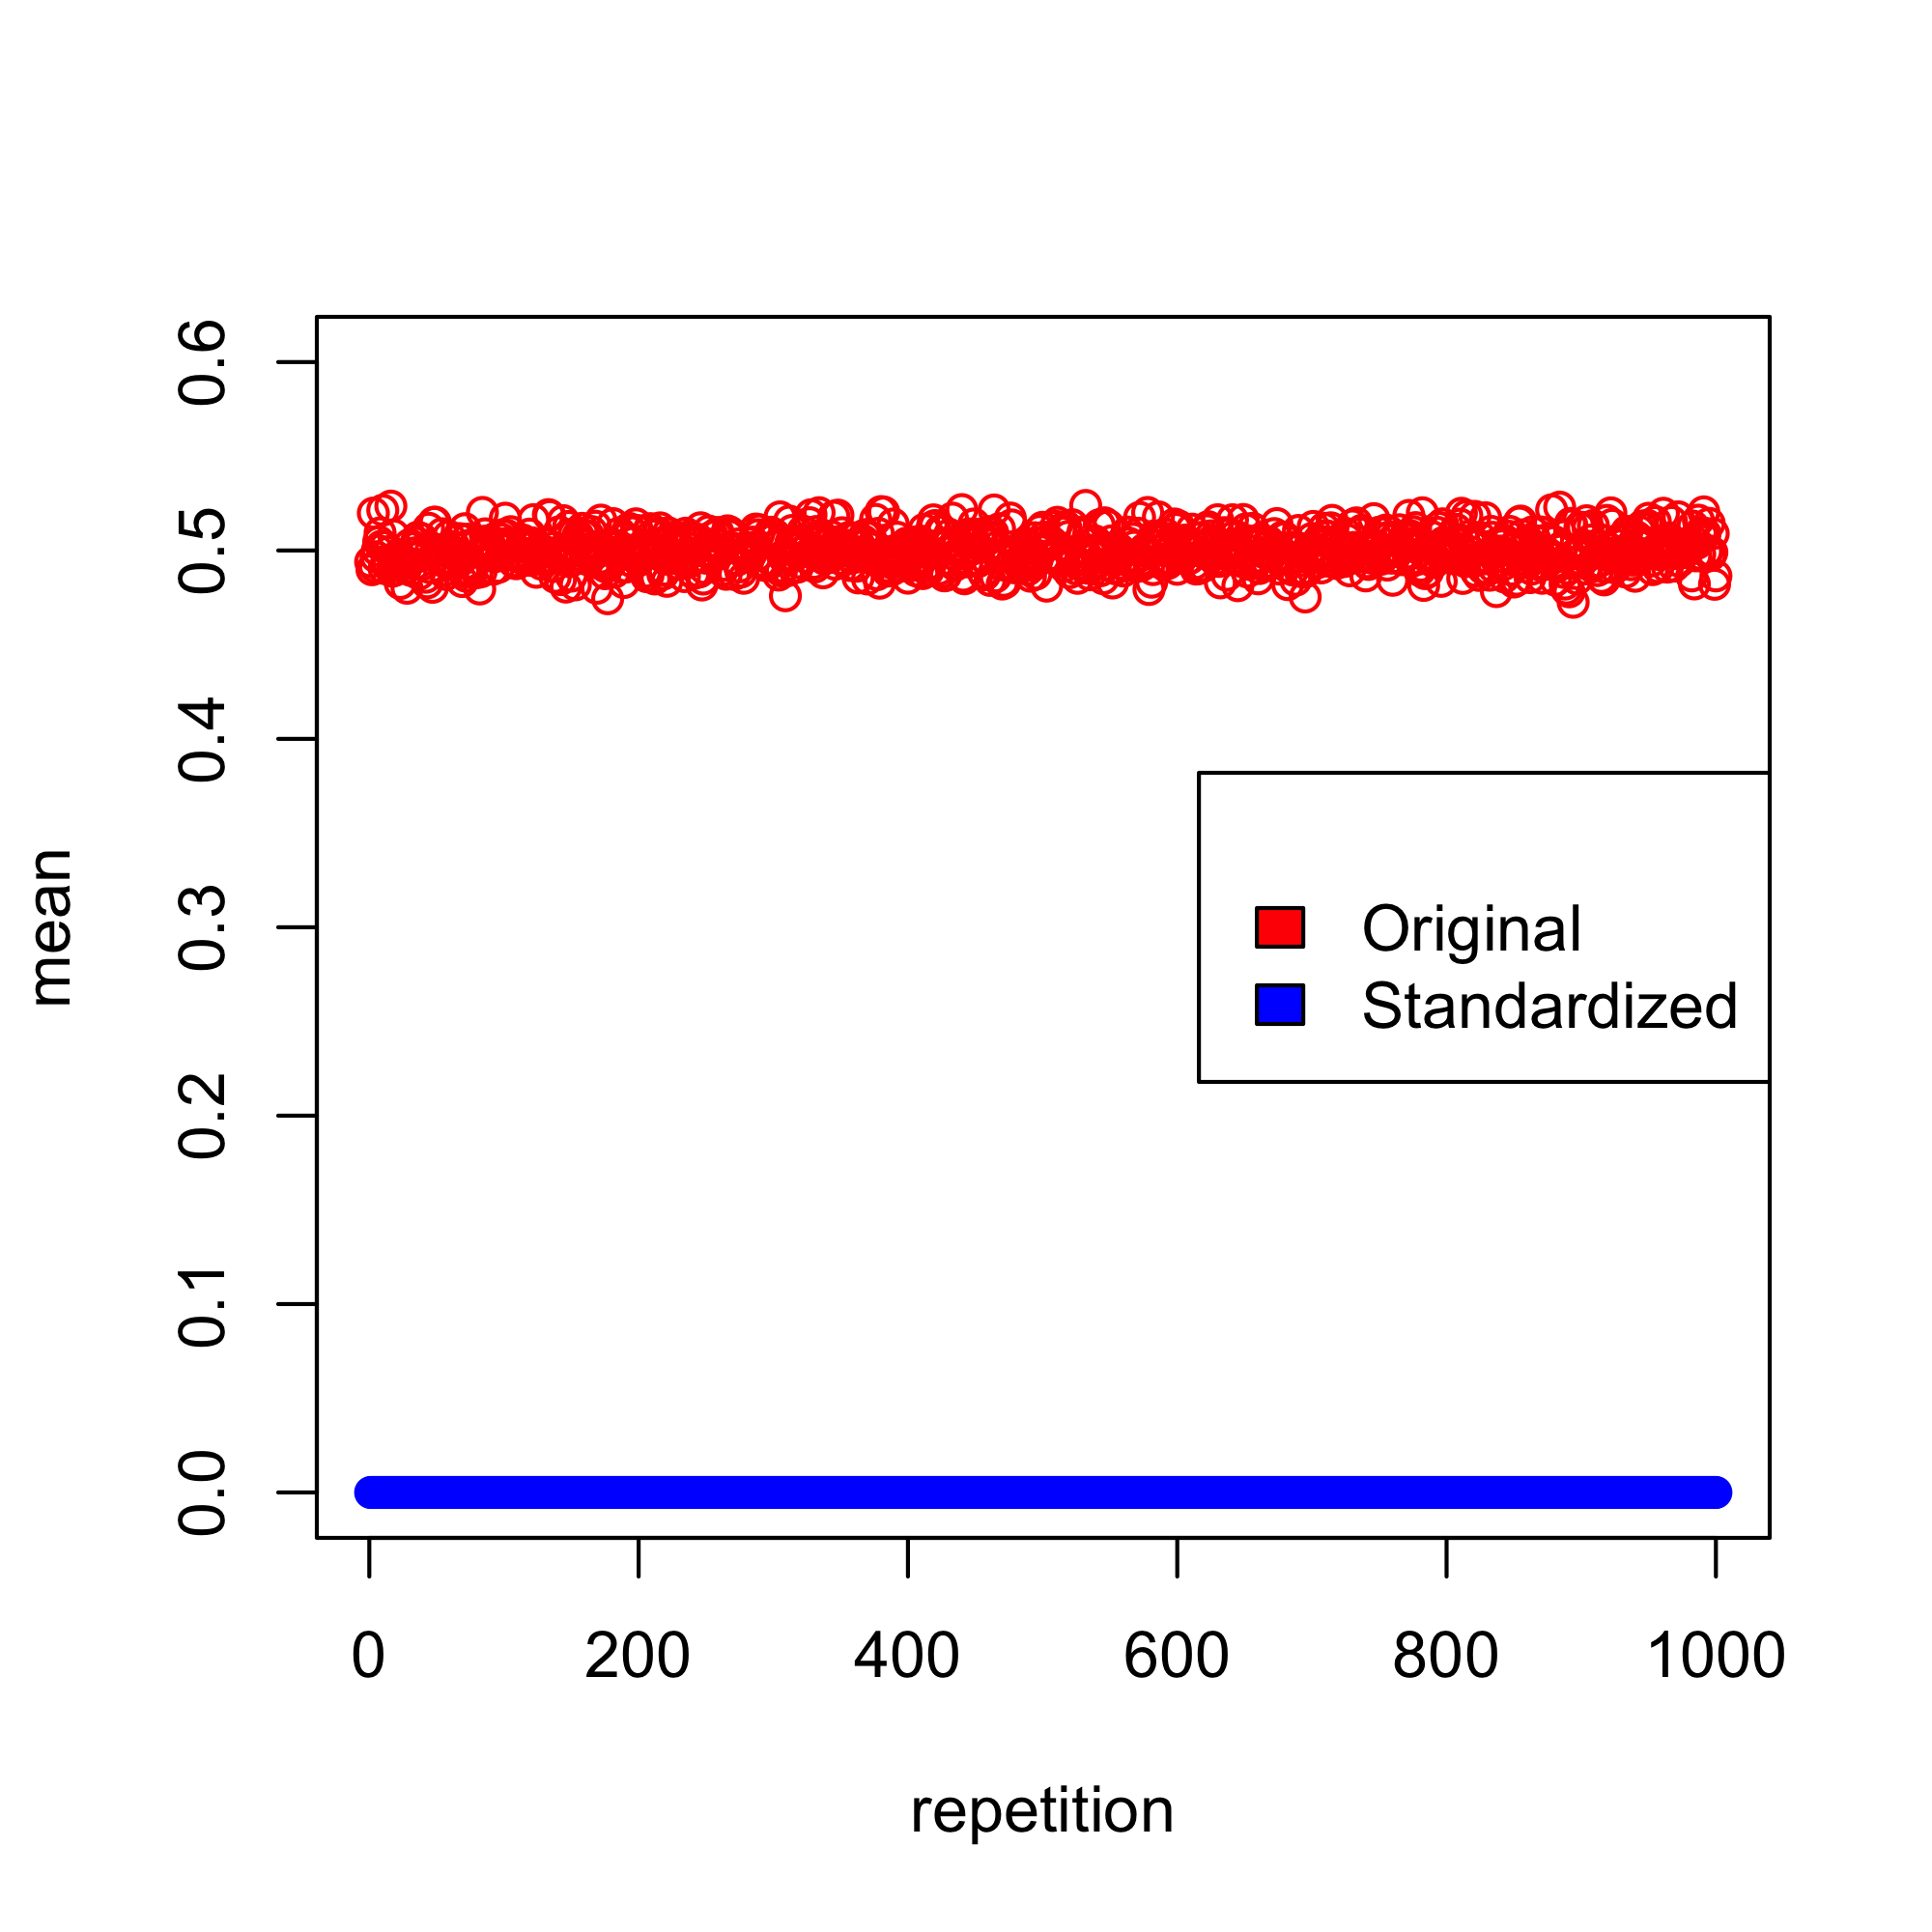
\includegraphics[width=\linewidth]{means_unif}
			\caption{Mean, with original numbers uniformly distributed.}
			\label{fig:means_unif}
		\end{subfigure}
		\hfill
		\begin{subfigure}{0.3\linewidth}
			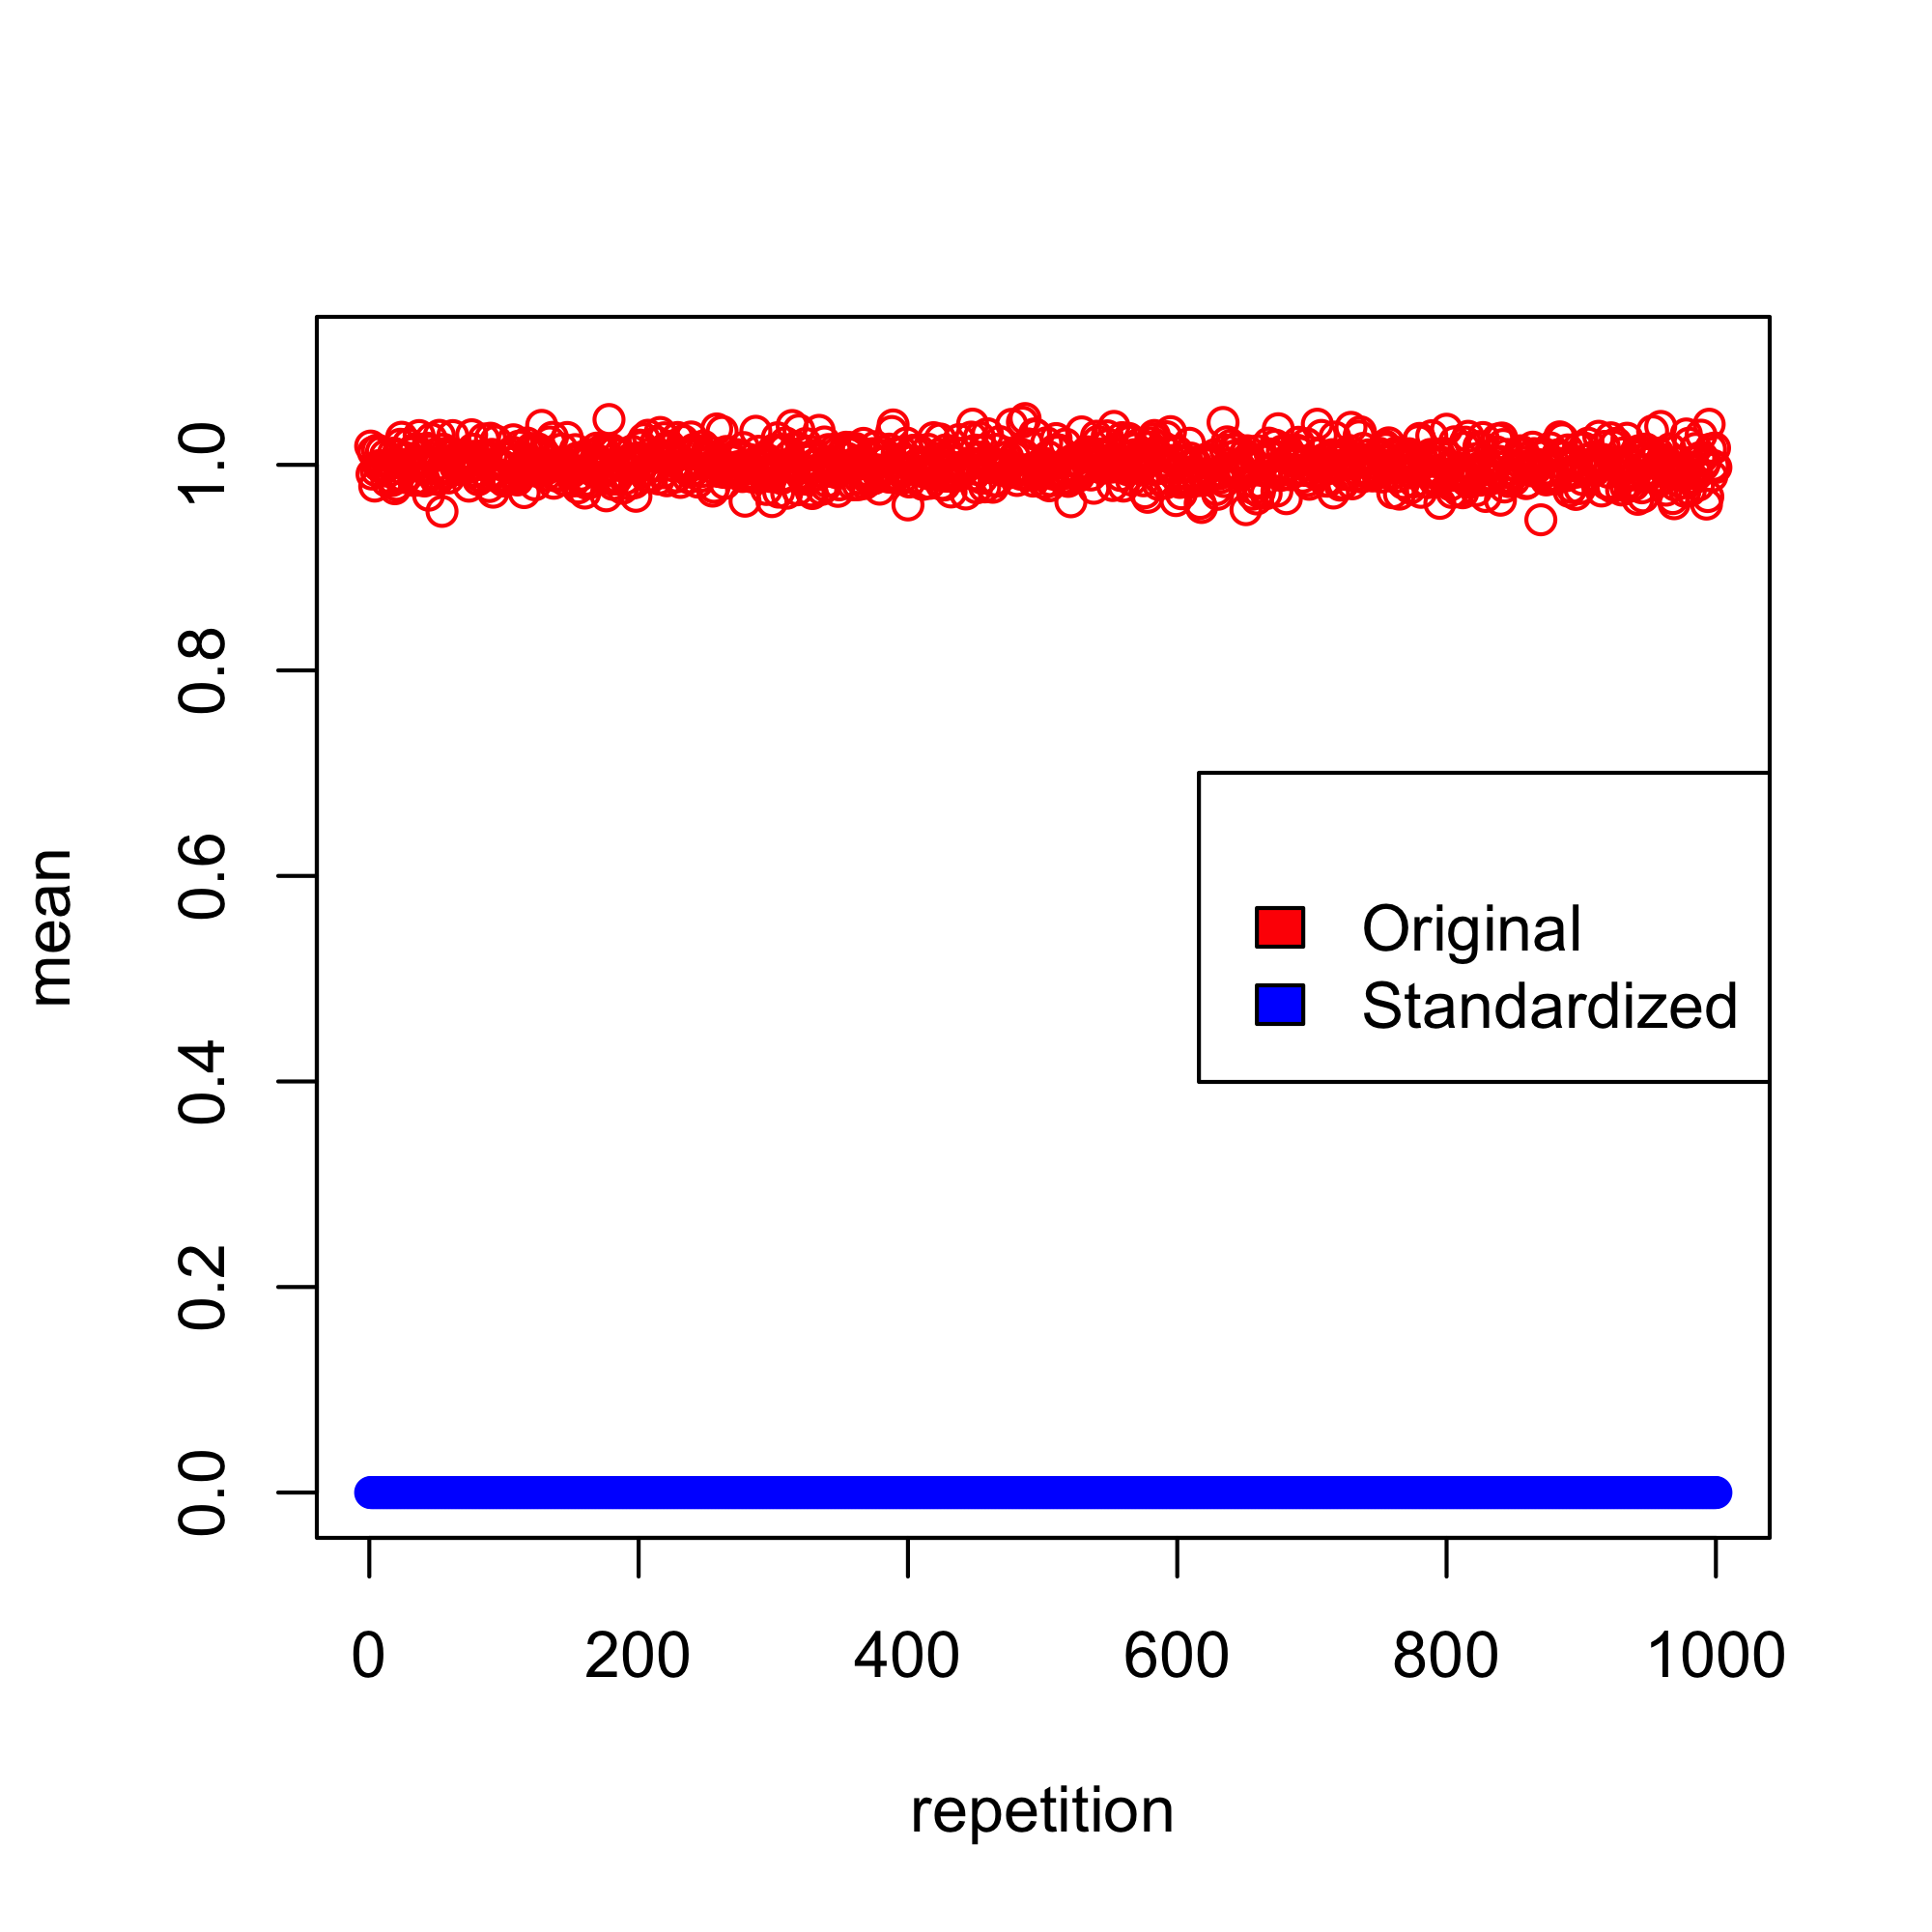
\includegraphics[width=\linewidth]{means_norm}
			\caption{Mean, with original numbers normally distributed.}
			\label{fig:means_norm}
		\end{subfigure}
		\hfill
		\begin{subfigure}{0.3\linewidth}
			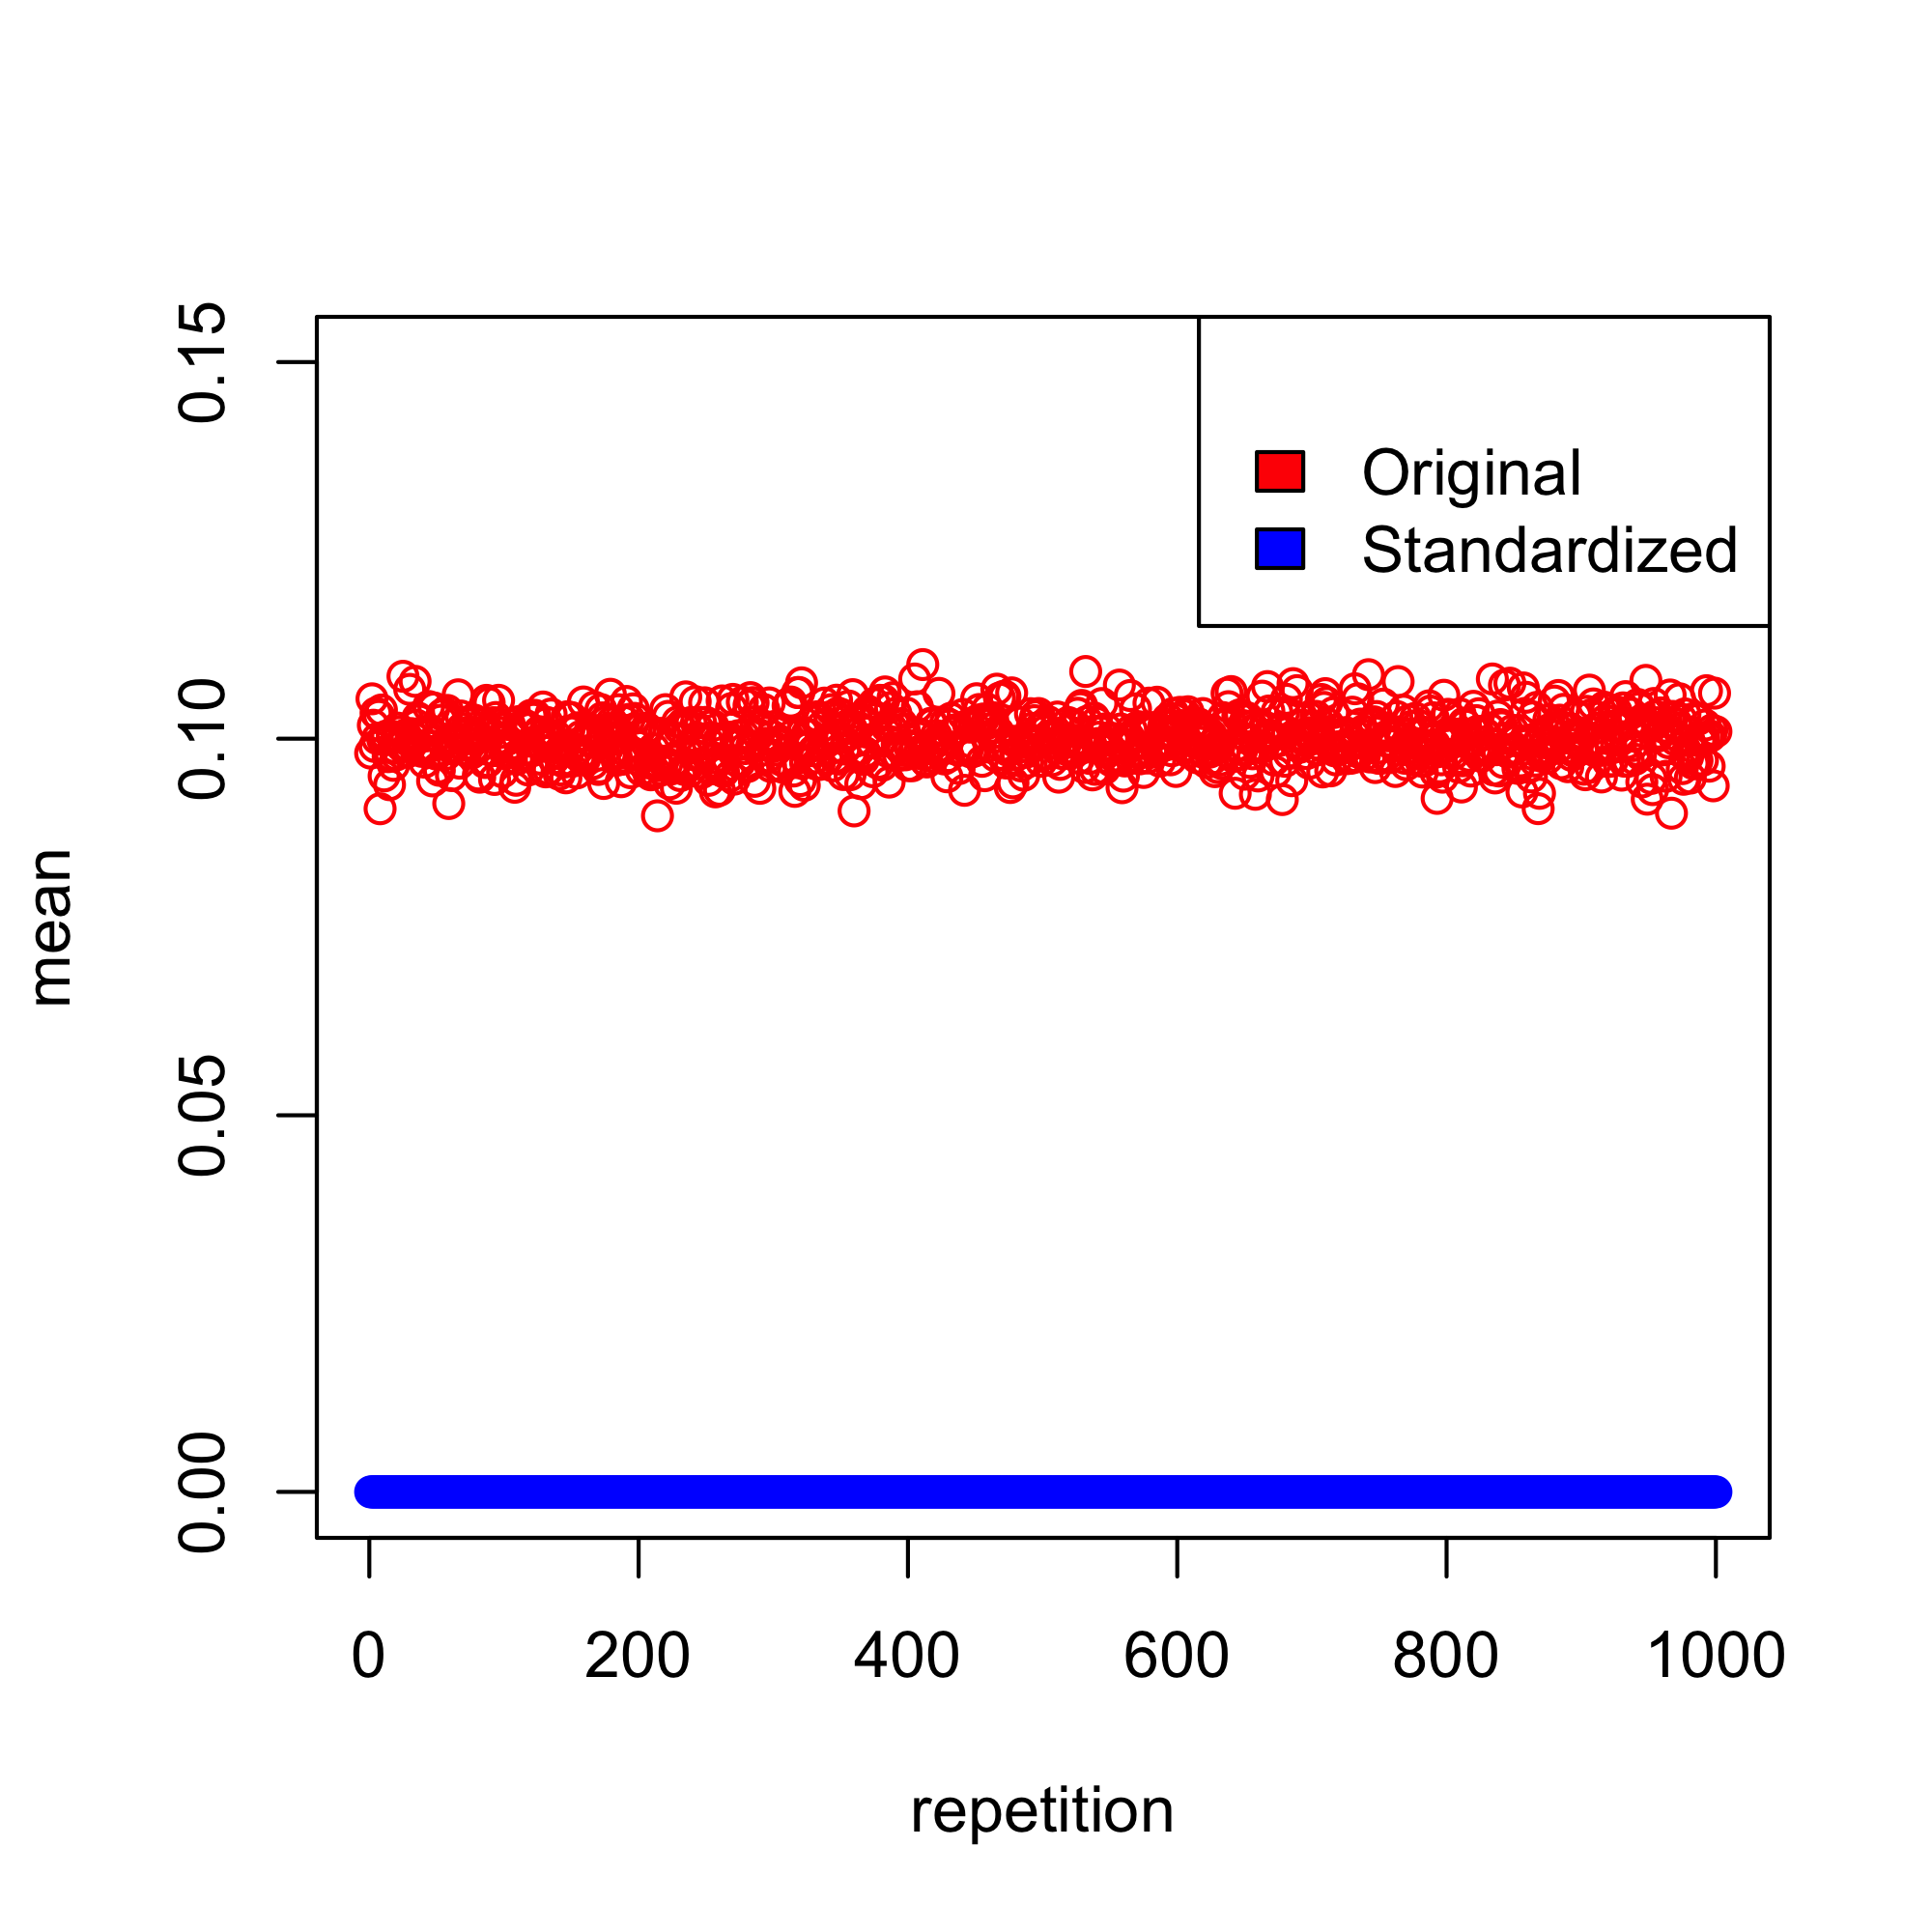
\includegraphics[width=\linewidth]{means_exp}
			\caption{Mean, with original numbers exponentially distributed.}
			\label{fig:means_exp}
		\end{subfigure}
		\hfill
		\begin{subfigure}{0.3\linewidth}
			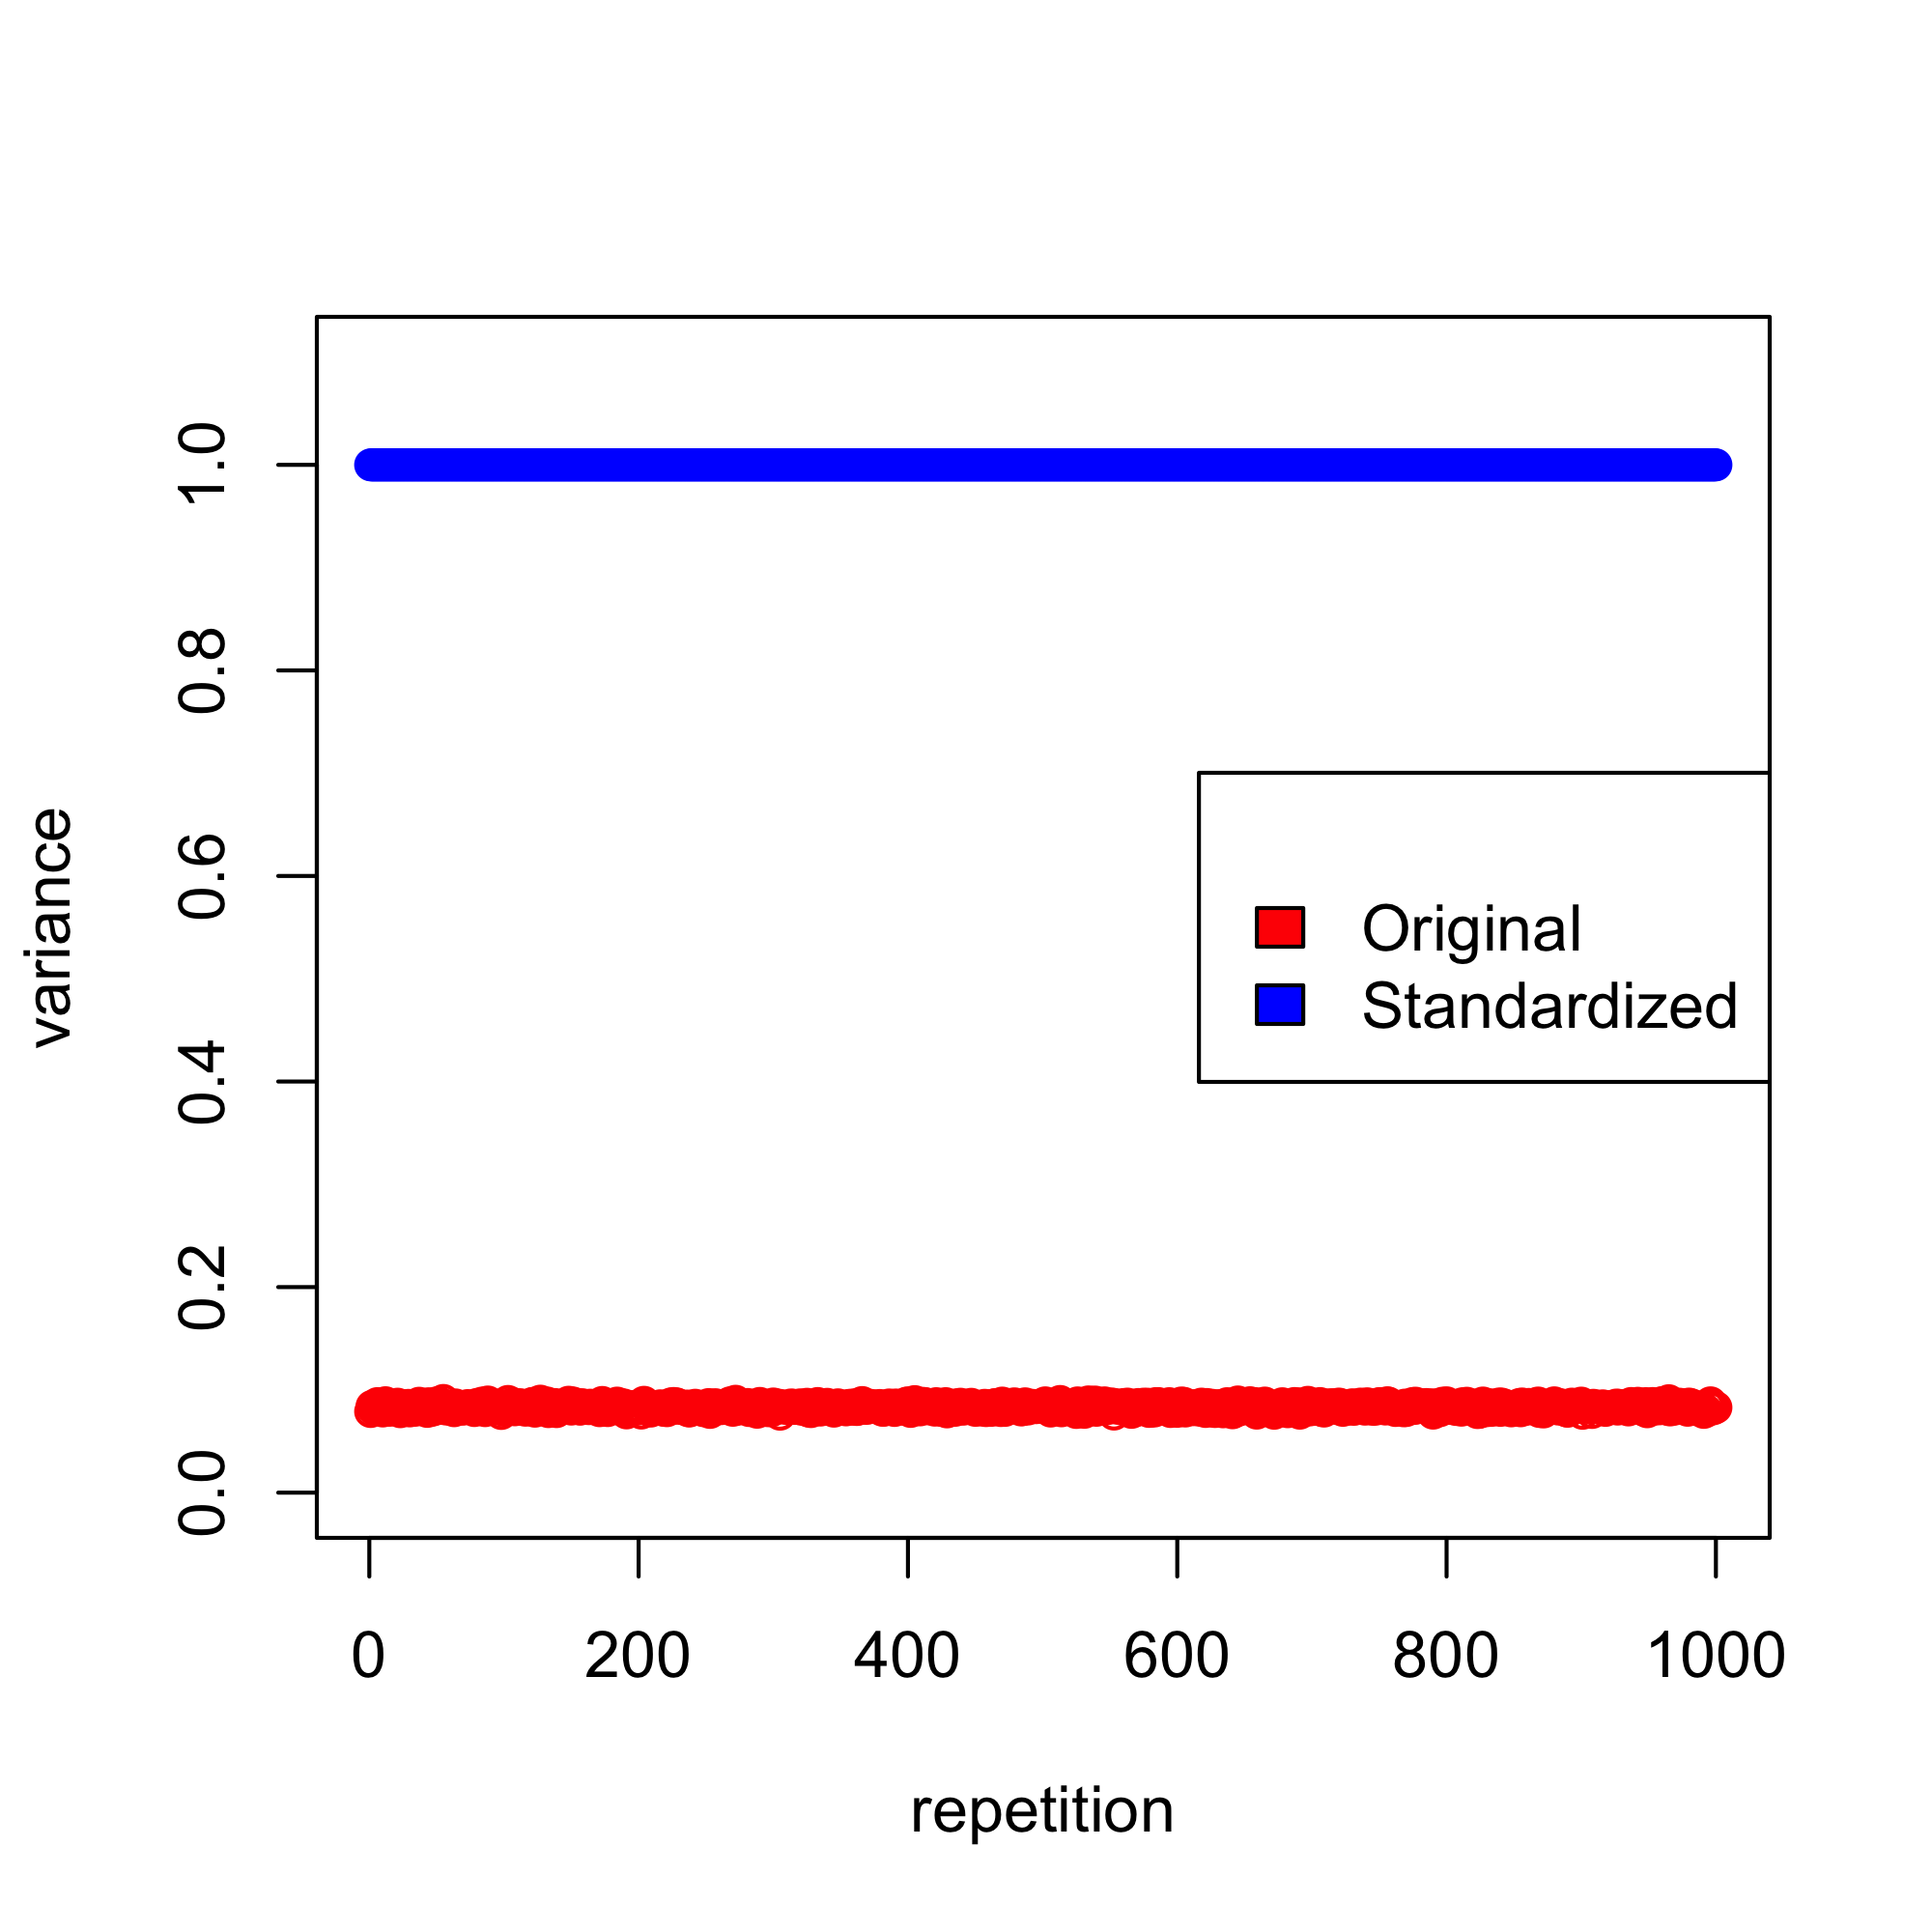
\includegraphics[width=\linewidth]{vars_unif}
			\caption{Variance, with original numbers uniformly distributed.}
			\label{fig:vars_unif}
		\end{subfigure}
		\hfill
		\begin{subfigure}{0.3\linewidth}
			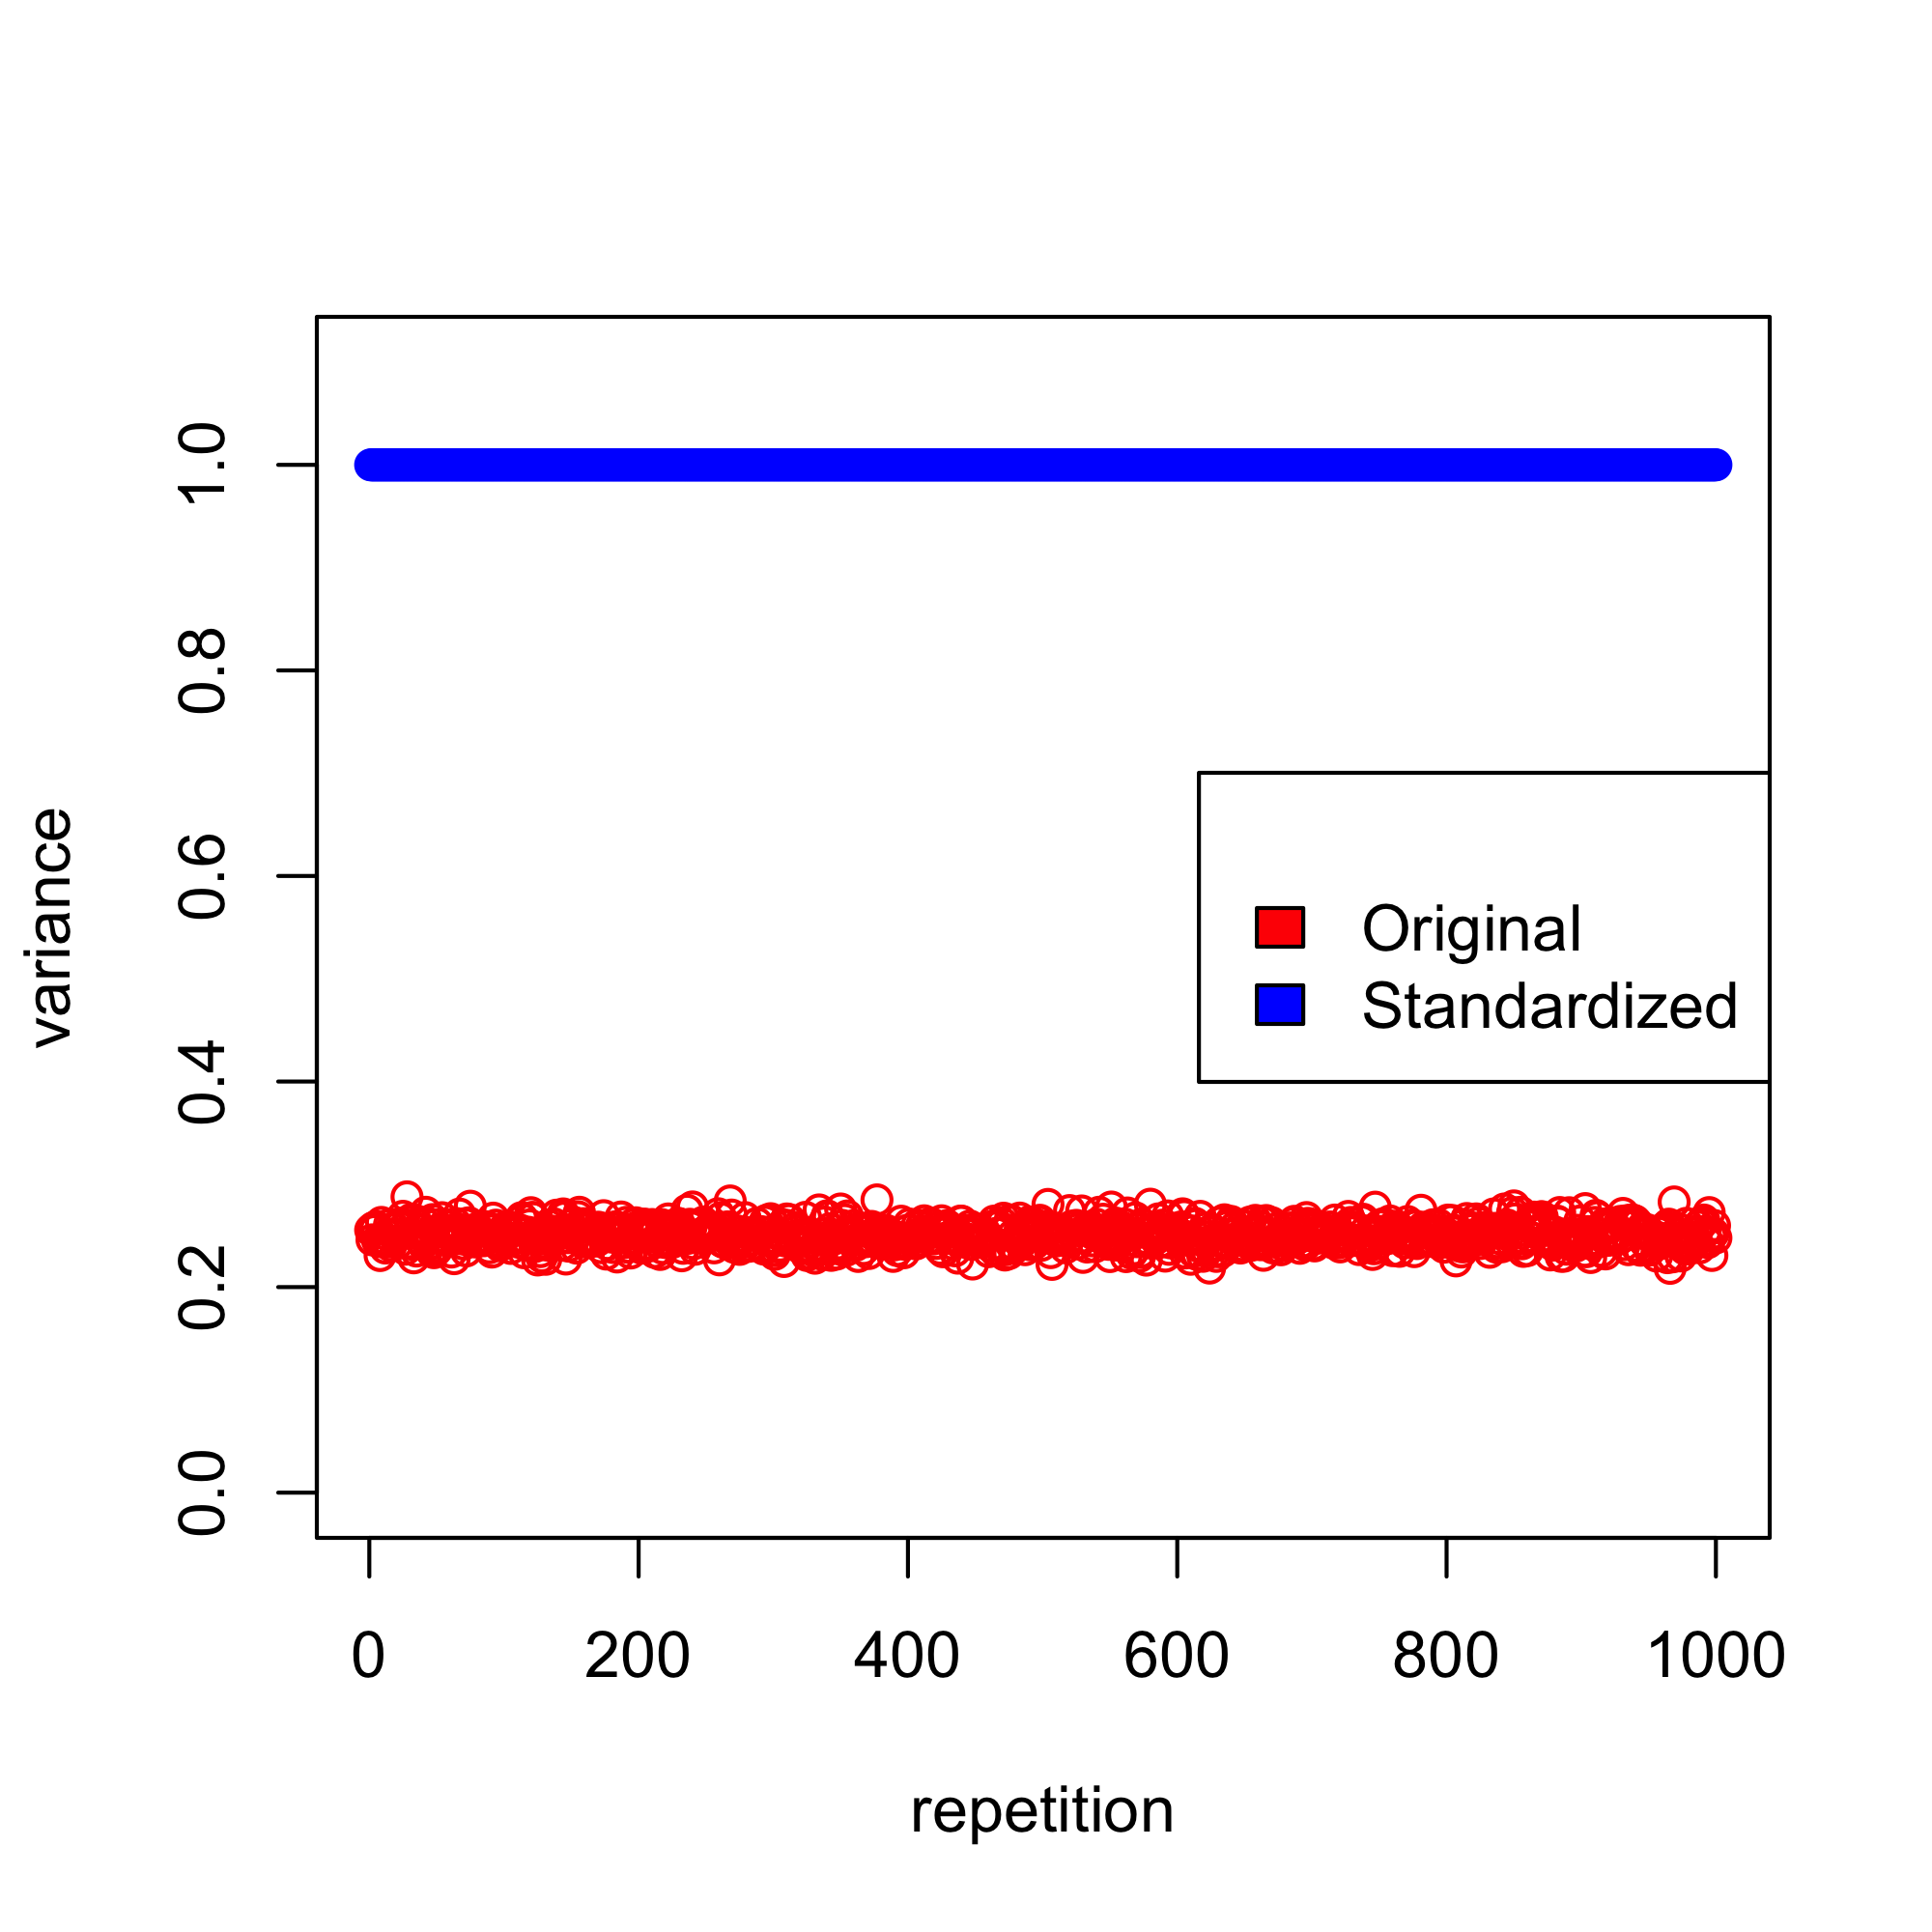
\includegraphics[width=\linewidth]{vars_norm}
			\caption{Variance, with original numbers normally distributed.}
			\label{fig:vars_norm}
		\end{subfigure}
		\hfill
		\begin{subfigure}{0.3\linewidth}
			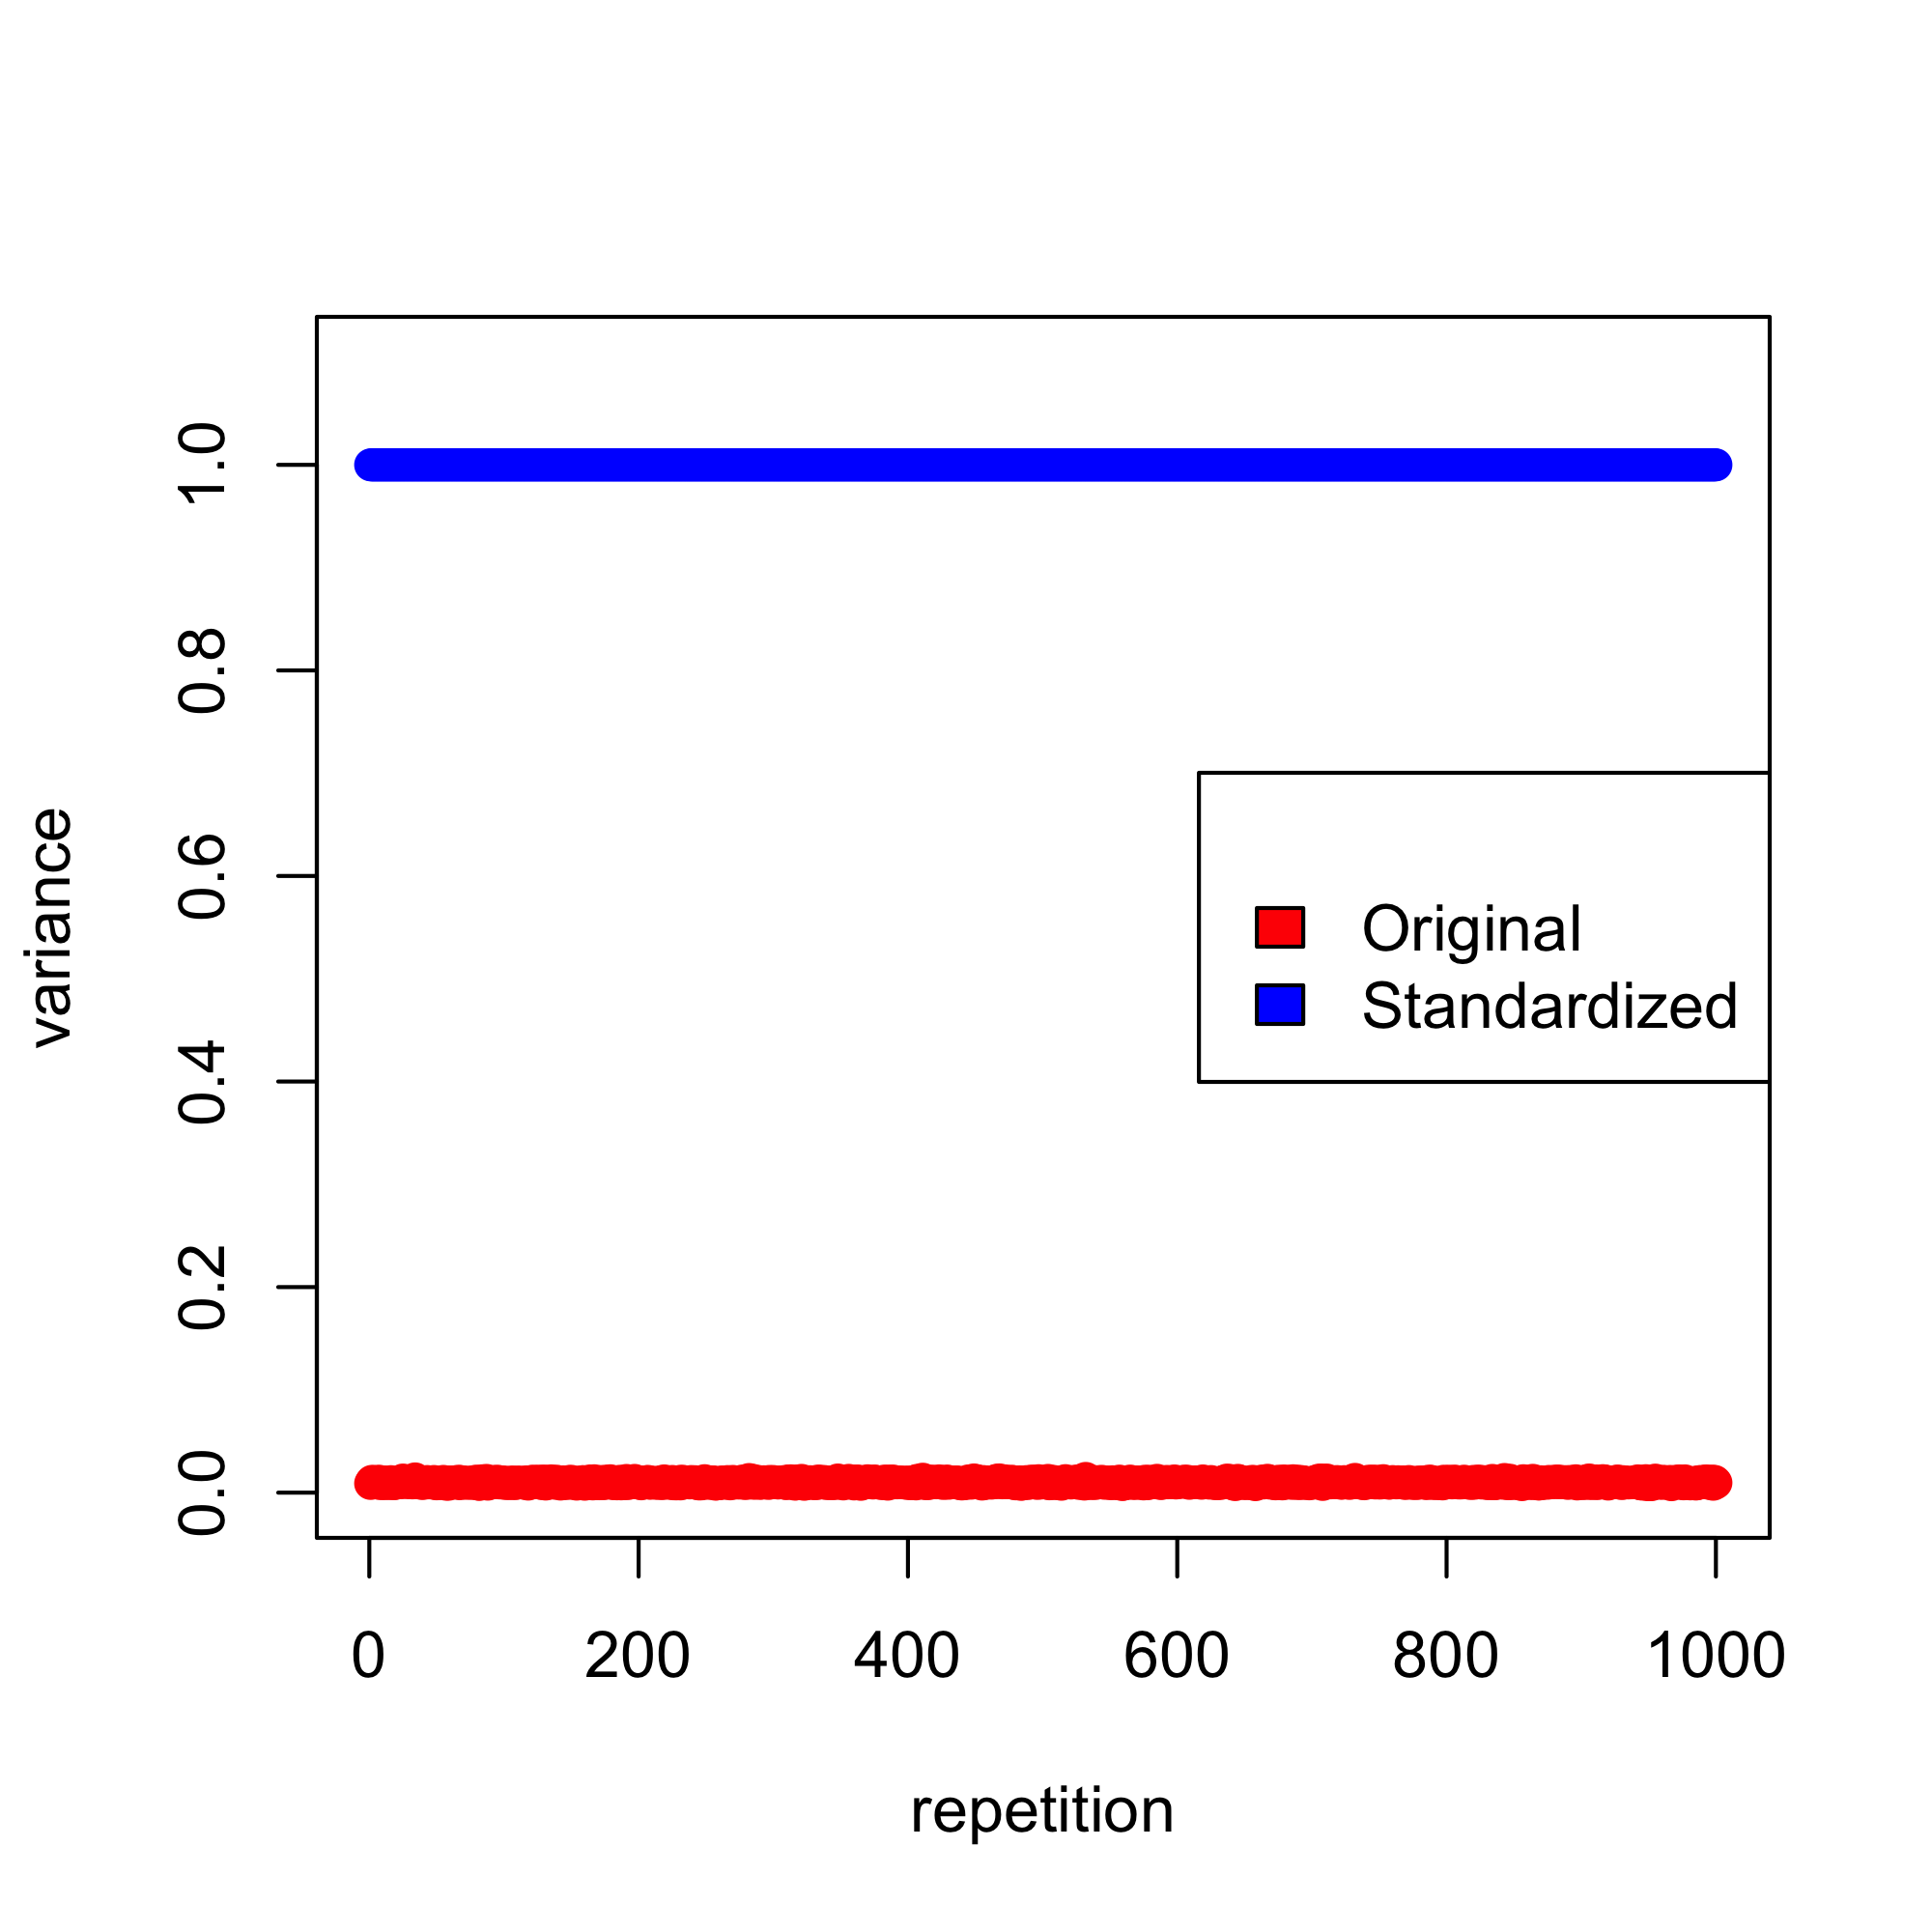
\includegraphics[width=\linewidth]{vars_exp}
			\caption{Variance, with original numbers exponentially distributed.}
			\label{fig:vars_exp}
		\end{subfigure}
		\caption{Mean and variance  before and after standardizing, Exercise \ref{ex:standardized}.} 
		\label{fig:standardized}
	\end{figure}
\end{proof}

\begin{ex}[Ex. 3, p. 278]\label{ex:lifetime}
	The lifetime, measured in hours, of the ACME super light bulb is a random variable $T$ with density function $f_T (t) = \lambda^2 t e^{-\lambda t}$, where $\lambda = 0.05$. What is the expected lifetime of this light bulb? What is its variance?
\end{ex}
\begin{proof}[Computer simulation]
	Analytically, it can be shown the light bulb has an expected lifetime of 40 hours, with a variance of 800. In order to simulate the lifetime of the light bulb, a thousand random numbers with density $f_T (t) = \lambda^2 t e^{-\lambda t}$ were generated, and its mean and variance computed. This was repeated a thousand times, storing the mean and variance in each repetition. On average, the mean was 40.138 and the variance 798.26. The computations were performed with the code in Listings \ref{lst:lifetime}. The mean and variance obtained in each repetition are shown in the boxplot in Figure \ref{fig:lifetime}.
	
	\begin{lstlisting}[language=R, caption={Code for Exercise \ref{ex:lifetime}.}, label={lst:lifetime} ]
library(distr)
p    <- function(x){ (0.05**2) * (x*exp(-0.05*x)) } # probability density function
dist <-AbscontDistribution(d=p)  # signature for a dist with pdf ~ p
rdist <- r(dist)                 # function to create random variates from p

mean_x <- numeric()
var_x <- numeric()

for (i in 1:1000){
	X <- rdist(1000)
	mean_x <- c(mean_x, mean(X))
	var_x <- c(var_x, var(X))
}
	\end{lstlisting}
	
	\begin{figure}
		\centering
		\begin{subfigure}{0.45\linewidth}
			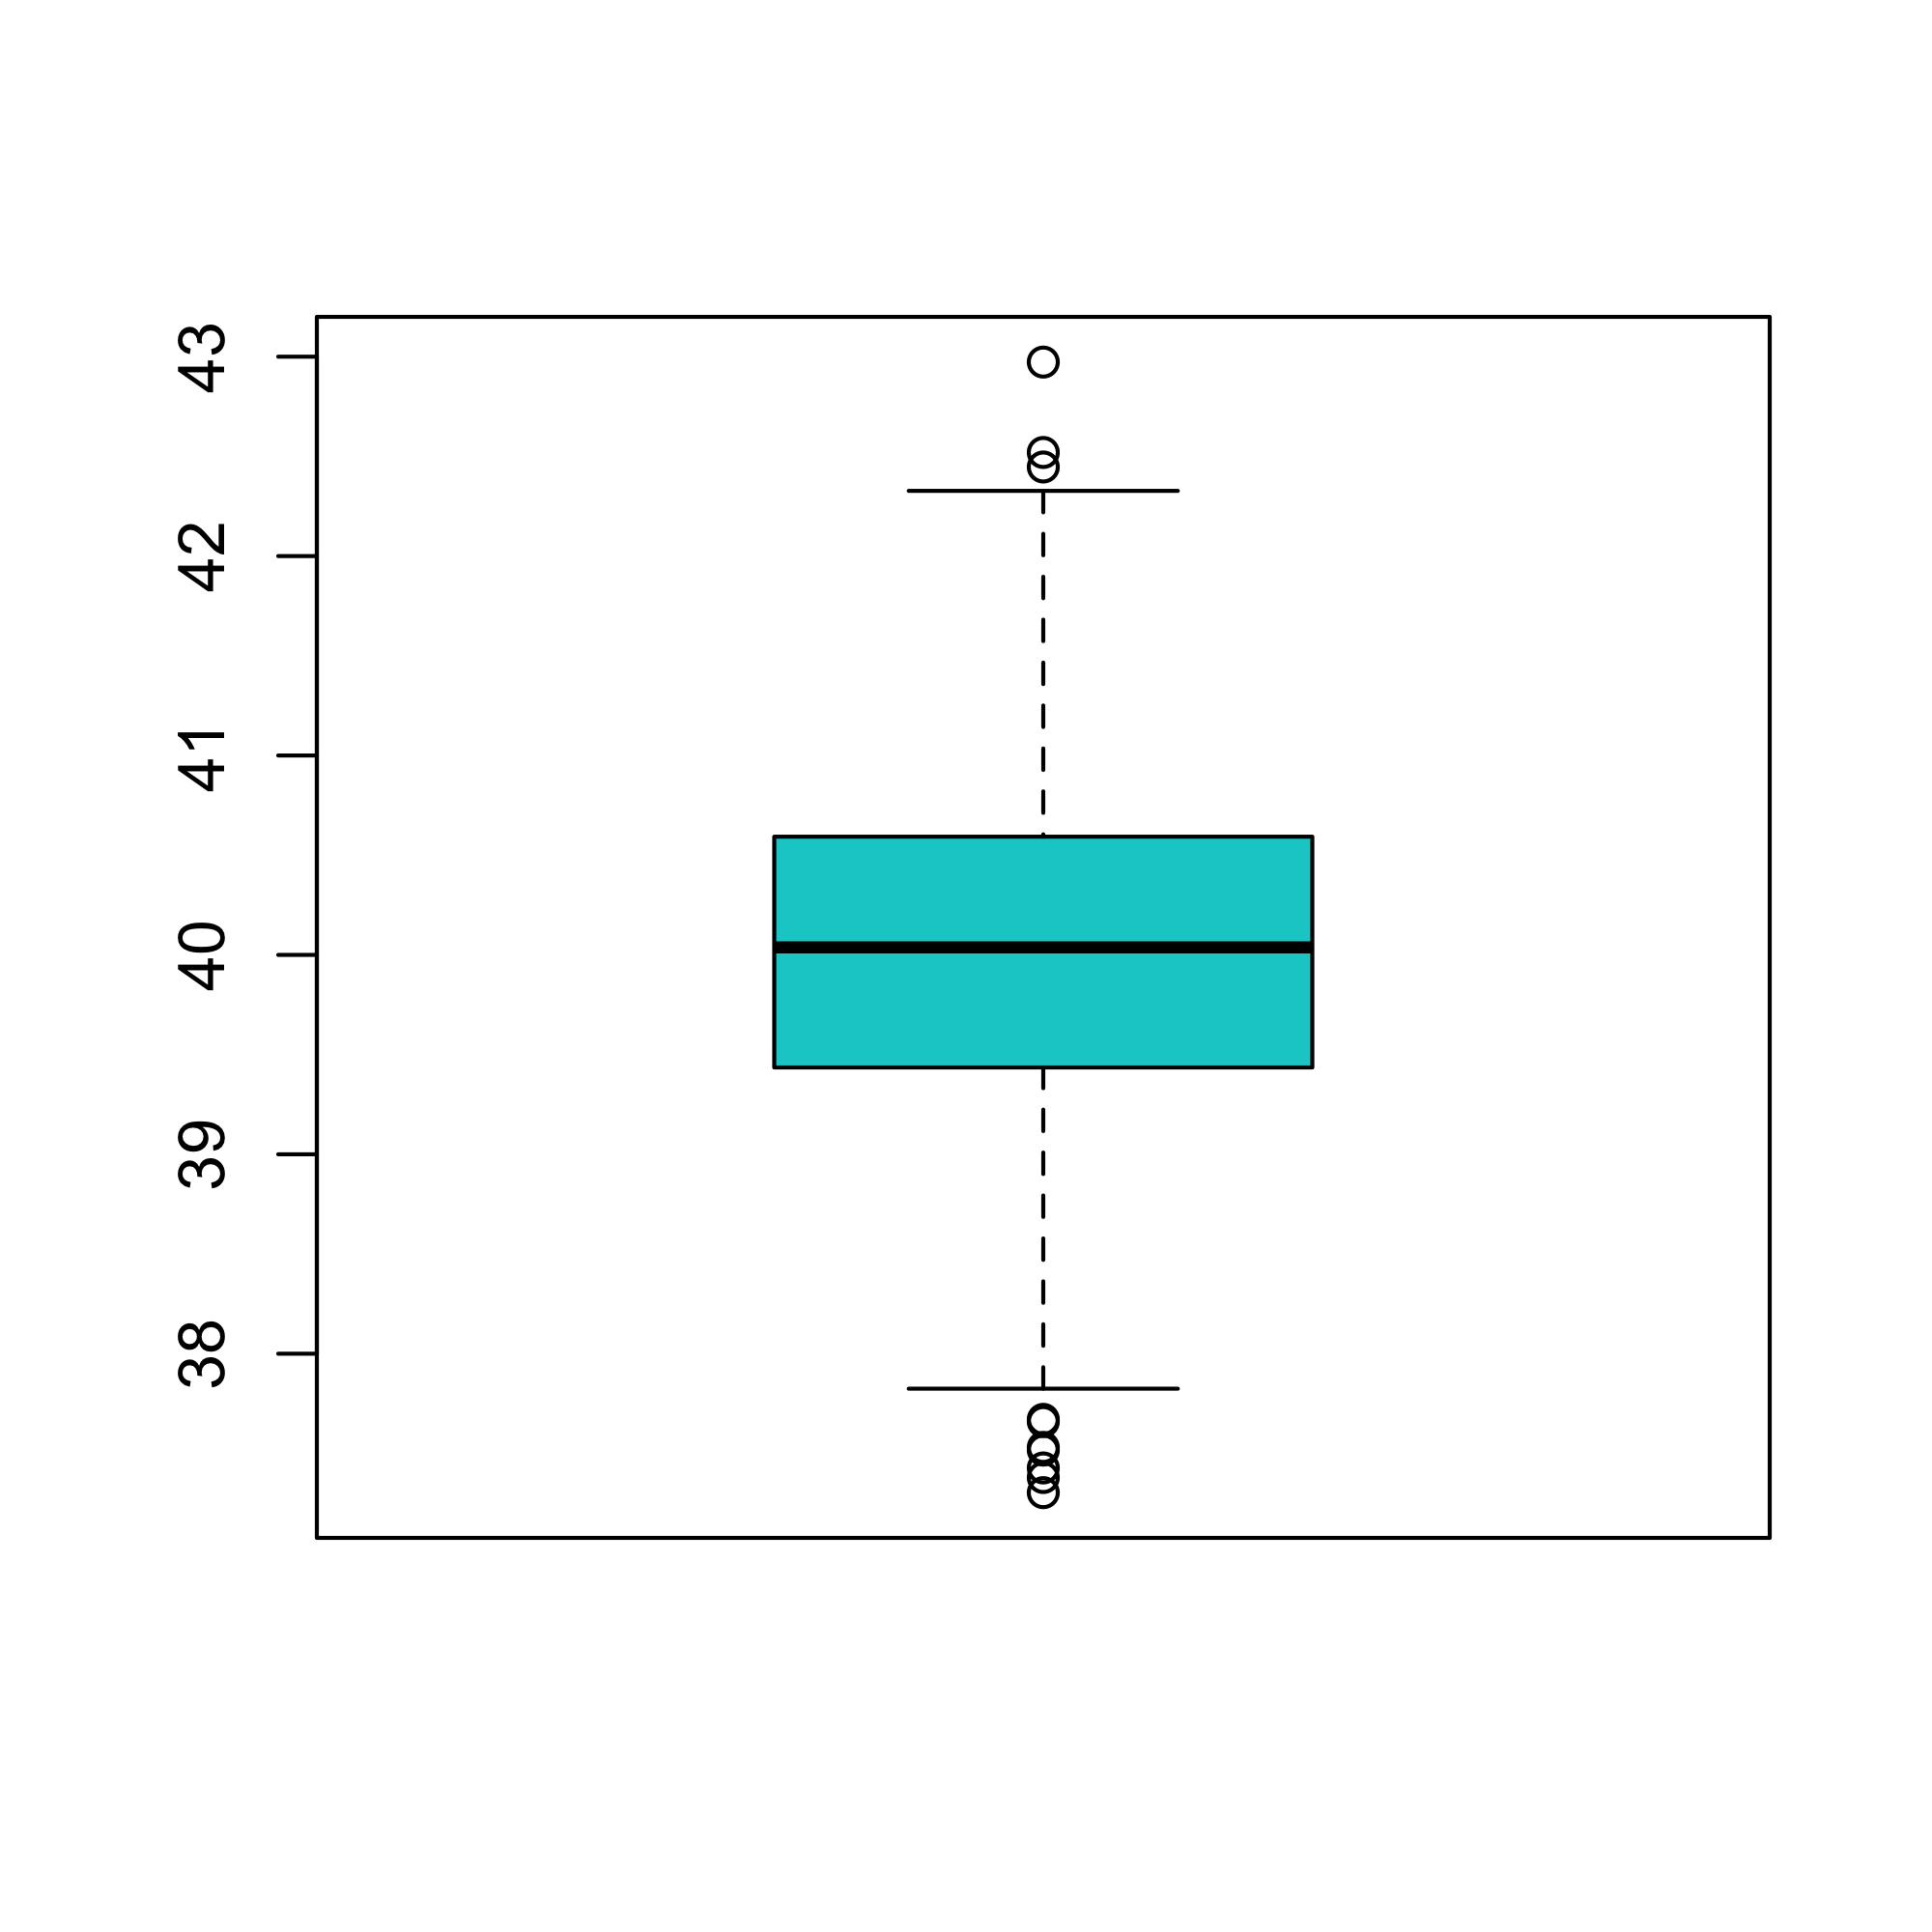
\includegraphics[width=\linewidth]{lifetime_mean}
			\caption{Mean in repetitions.}
			\label{fig:lifetime_mean}
		\end{subfigure}
		\hfill
		\begin{subfigure}{0.45\linewidth}
			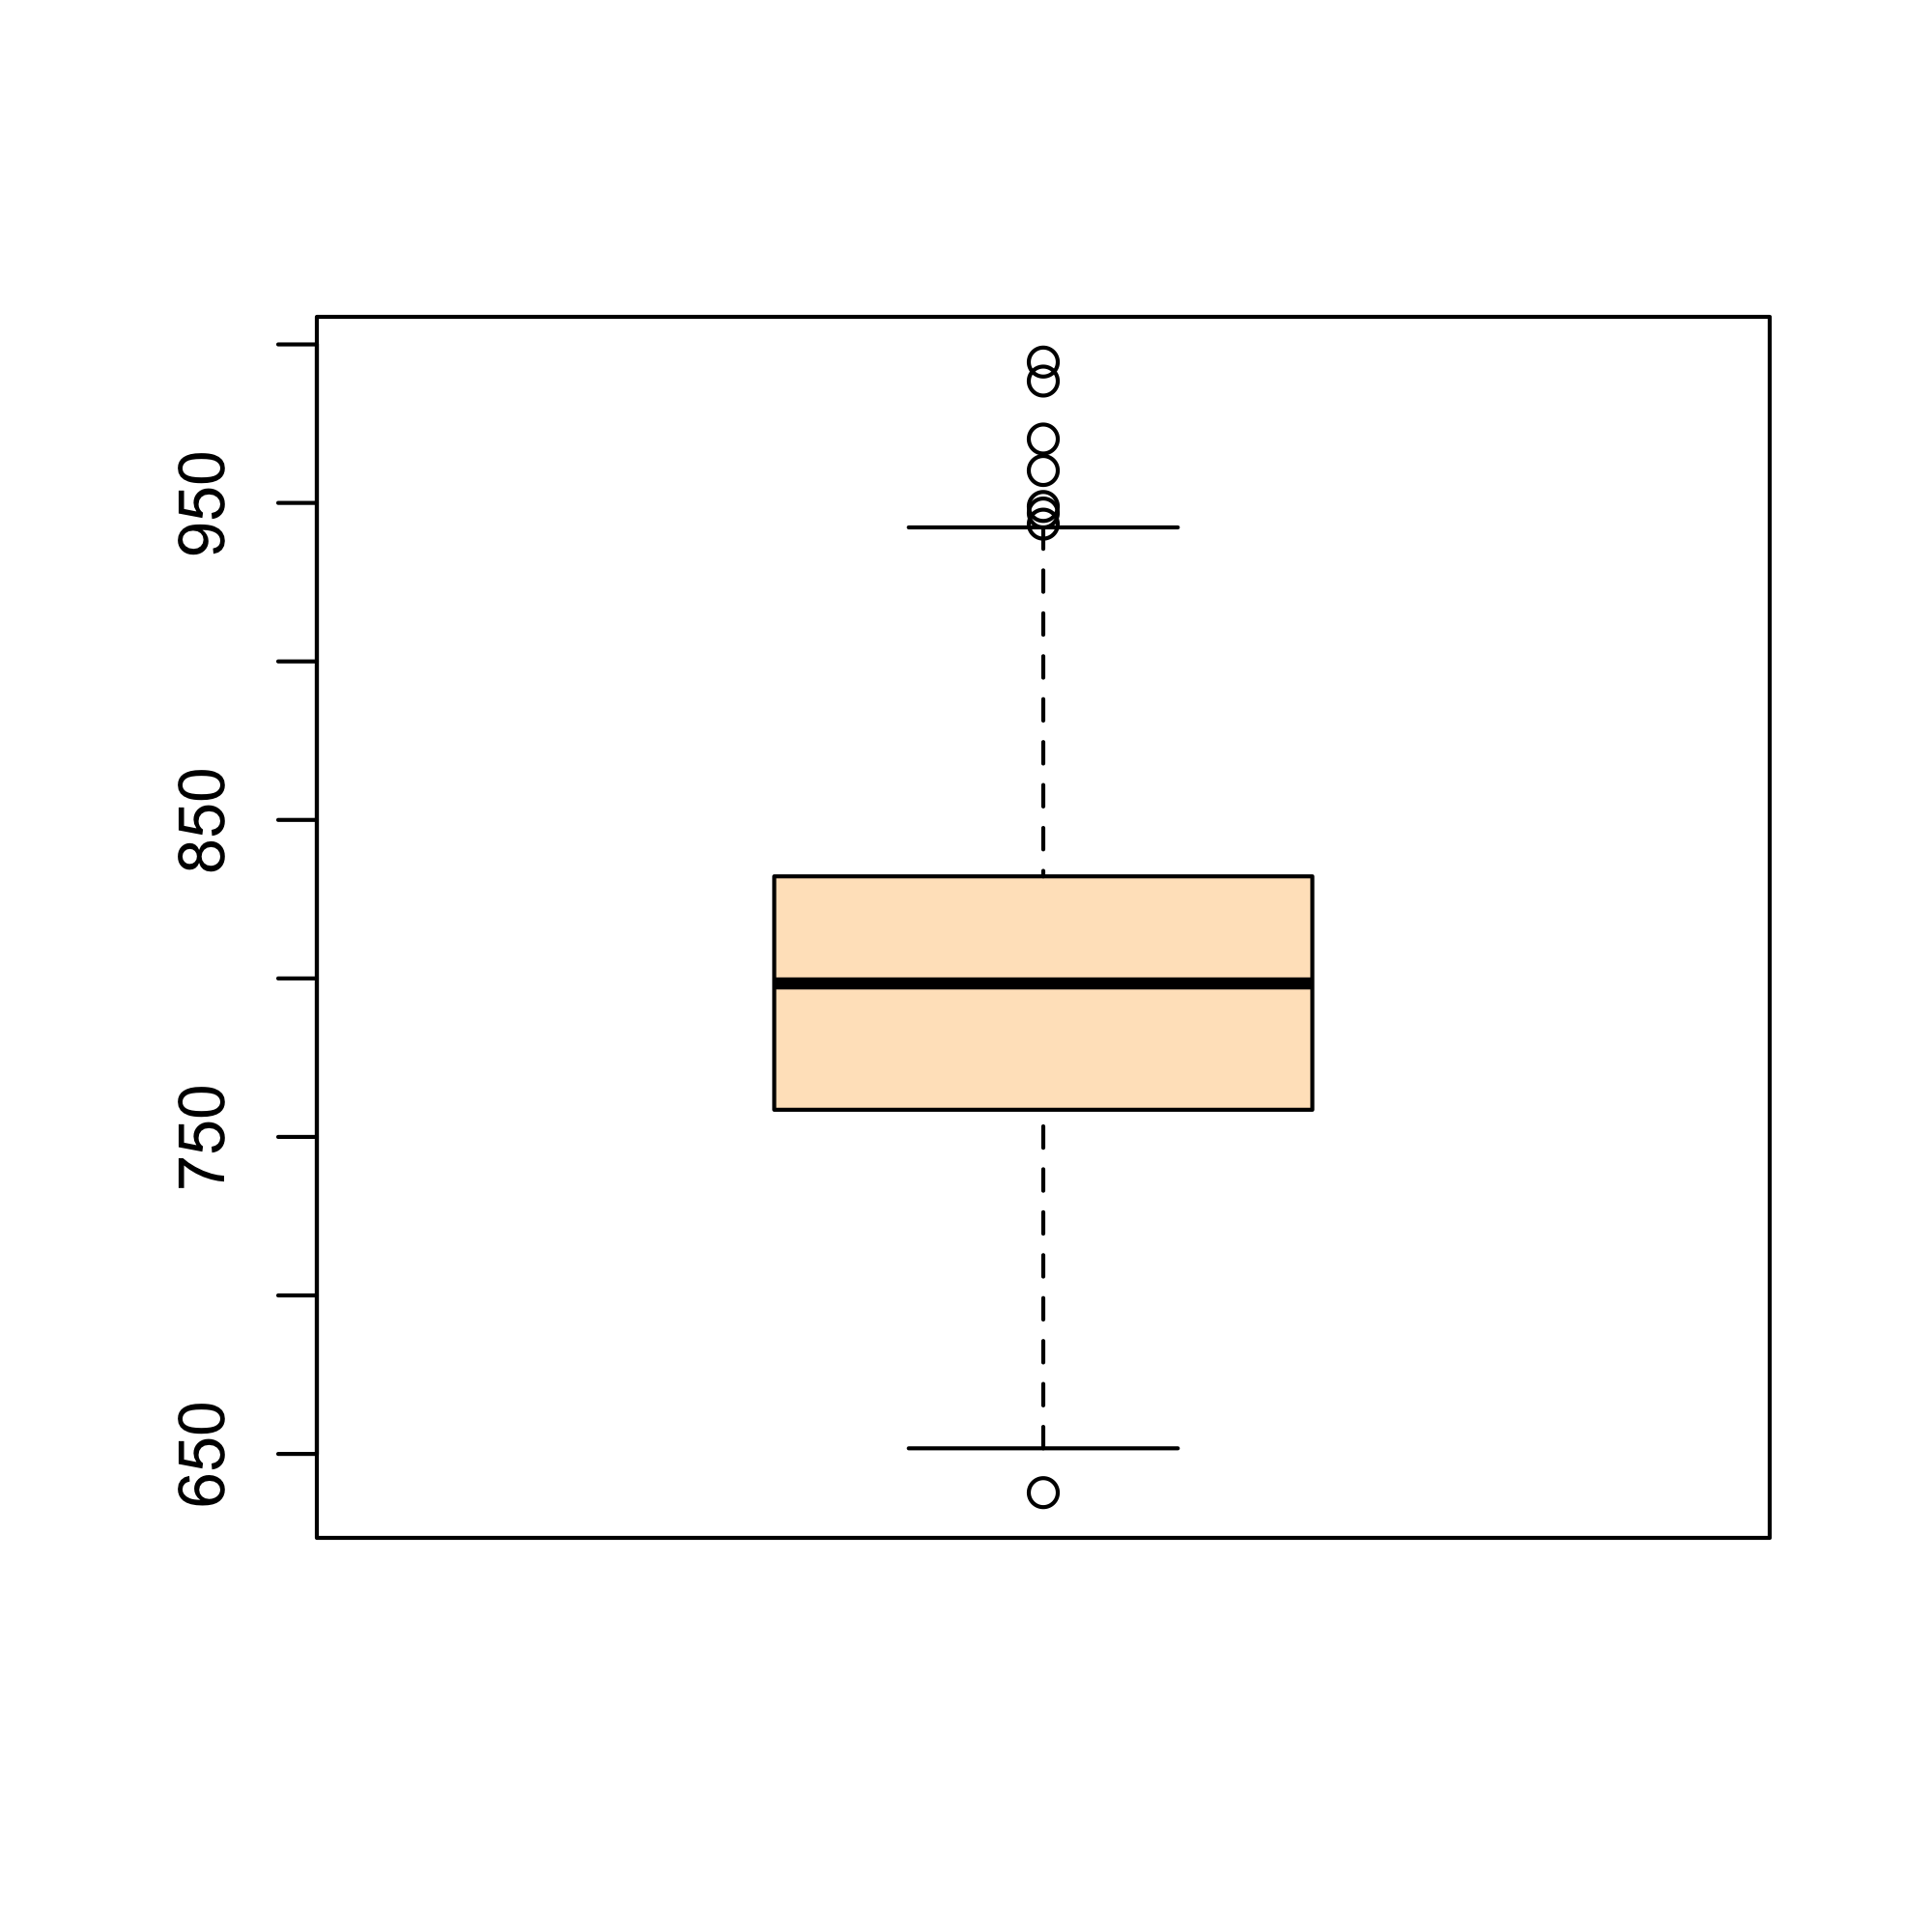
\includegraphics[width=\linewidth]{lifetime_variance}
			\caption{Variance in repetitions.}
			\label{fig:lifetime_variance}
		\end{subfigure}
		\caption{Mean and variance in the experiment repetitions for Exercise \ref{ex:lifetime}.} 
		\label{fig:lifetime}
	\end{figure}
	
\end{proof}

\begin{ex}[Ex. 1, p. 247]\label{ex:cards_drawn}
	A card is drawn at random from a deck consisting of cards numbered 2 through 10. A player wins 1 dollar if the number on the card is odd and loses 1 dollar if the number is even. What is the expected value of his winnings?
\end{ex}
\begin{proof}[Computer simulation]
We simulate 50,000 repetitions of the experiment, drawing a random card and storing the corresponding score. A mean of $-0.113$ is obtained from this experiment, while analytically the expected value is $-1/9 \approx -0.111$. The code used for the simulation is in Listing \ref{lst:cards_drawn}.

\begin{lstlisting}[language=R, caption={Code for Exercise \ref{ex:cards_drawn}.}, label={lst:cards_drawn} ]
cards = c(2, 3, 4, 5, 6, 7, 8, 9, 10)

winnings <- numeric()

for (i in 1:50000){
	drawn_card <- sample(cards,1)
	winnings <- c(winnings, 2*(drawn_card %% 2) - 1)
}
\end{lstlisting}
\end{proof}
%%%%%%%%%%%%%%%%%%%%%%%%%%%%%%%%%%%%%%%%%%%%%%%%%%%%%%%%%%%%%%%%%%%%%%%%%%%%%%%%

\bibliography{ref}

\end{document}
